%!Mode::"TeX:UTF-8"
\documentclass[12pt,a4paper]{ctexart}
\usepackage{graphicx}
\usepackage{float}
\usepackage{amsmath}
\usepackage{listings}
\usepackage{amssymb}
\usepackage{url}
\usepackage{geometry}
\geometry{a4paper,centering,scale=0.8}
\usepackage[format=hang,font=small,textfont=it]{caption}
\usepackage[nottoc]{tocbibind}
\usepackage{listings}
\usepackage{xcolor}

\lstset{
	numbers=left, 
	numberstyle= \tiny, 
	keywordstyle= \color{ blue!70},
	commentstyle= \color{red!50!green!50!blue!50}, 
	frame=shadowbox, % 阴影效果
	rulesepcolor= \color{ red!20!green!20!blue!20} ,
	escapeinside=``, % 英文分号中可写入中文
	xleftmargin=2em,xrightmargin=2em, aboveskip=1em,
	framexleftmargin=2em
} 

\lstset{
	columns=fixed,       
	numbers=left,                                        % 在左侧显示行号
	numberstyle=\tiny\color{gray},                       % 设定行号格式
	frame=none,                                          % 不显示背景边框
	backgroundcolor=\color[RGB]{245,245,244},            % 设定背景颜色
	keywordstyle=\color[RGB]{40,40,255},                 % 设定关键字颜色
	numberstyle=\footnotesize\color{darkgray},           
	commentstyle=\it\color[RGB]{0,96,96},                % 设置代码注释的格式
	stringstyle=\rmfamily\slshape\color[RGB]{128,0,0},   % 设置字符串格式
	showstringspaces=false,                              % 不显示字符串中的空格
	language=c++,                                        % 设置语言
}
	
\title{\kaishu \Huge 从一种叫Astrojax的玩具讲起}
\date{}
\begin{document}
	\maketitle
	\begin{figure}[h] %figure环境,h默认参数是可以浮动,不是固定在当前位置。如果要不浮动,你就可以使用大写float宏包的H参数,固定图片在当前位置,禁止浮动。
		\centering %使图片居中显示
		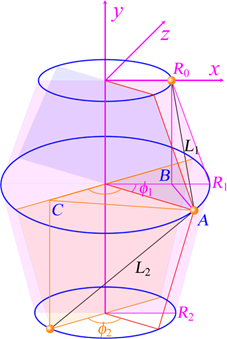
\includegraphics[scale=2.5]{T07.png} %中括号中的参数是设置图片充满文档的大小,你也可以使用小数来缩小图片的尺寸。
		%\caption{狼伴归途} %caption是用来给图片加上图题的
		%\label{wolf} %这是添加标签,方便在文章中引用图片。
	\end{figure}%figure环境
	
	
	\clearpage
	\renewcommand{\baselinestretch}{0.9}
	
	\begin{abstract}
		Astrojax又称"太空悠悠球",是一款风靡全美国的玩具,其结构类似于双摆,但又有明显不同——中间球可以沿着绳子滑动。目前国际上对于双摆的研究较为成熟,仿真多样,但是对于Astrojax这款新兴玩具的仿真和稳定状态的研究还几乎是空白。本文重点研究了Astrojax的水平轨道稳定态和仿真算法。Astrojax的稳定状态类似于弹簧振子的稳定受迫运动状态,即系统能量的输入和输出相等,系统达到稳定状态,因此我们从弹簧振子讲起,再从单摆过渡到astrojax。我们的仿真模型是基于Unity3D开发的,背后的物理模型我们使用C\# 进行构建,我们利用保辛算法对运动进行演化,得到了与实际相符的仿真结果,我们同时针对windows平台和Android平台发布了我们的仿真程序,这样大家就可以在自己的手机或者电脑上操纵Astrojax。

		\par\textbf{关键词: } Astrojax; 弹簧振子; Unity3D;稳定受迫振动%“\par在段首,表示另起一行,“\textbf{}”,花括号内的内容加粗显示
	\end{abstract}
	\newpage%另起一页
	\clearpage
	\renewcommand{\baselinestretch}{0.9}
	\thispagestyle{empty}
	\tableofcontents

	\clearpage
	\thispagestyle{empty}
	\section{Astrojax介绍}
	Astrojax是一款风靡全美国的玩具:将绳子穿过一个带有洞的球,这样球就可以沿着绳子自由移动。把另一个球系在绳子的一端。当你周期性地移动绳子的自由端时,你可以观察到两个球的复杂运动。此系统不同于双摆---中间的球可以沿着绳子自由滑动。因其运动类似于行星,故命名为Astrojax.
	
			\begin{figure}[h] %figure环境,h默认参数是可以浮动,不是固定在当前位置。如果要不浮动,你就可以使用大写float宏包的H参数,固定图片在当前位置,禁止浮动。
		\centering %使图片居中显示
		%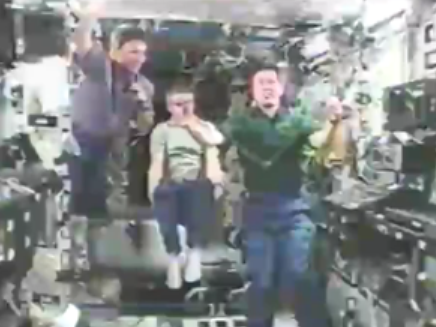
\includegraphics[scale=0.6]{T801.jpg} %中括号中的参数是设置图片充满文档的大小,你也可以使用小数来缩小图片的尺寸。
		%\caption{狼伴归途} %caption是用来给图片加上图题的
		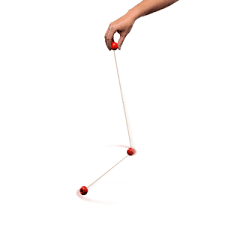
\includegraphics[scale=0.5]{T0102.png}
		%\label{wolf} %这是添加标签,方便在文章中引用图片。
	\end{figure}%figure环境\\
	
	Astrojax富含教育意义,美国太空总署NASA,将astrojax作为其【太空玩具】教育计划的一部分,并在2003年由宇航员带入太空进行了演示。
		\begin{figure}[h] %figure环境,h默认参数是可以浮动,不是固定在当前位置。如果要不浮动,你就可以使用大写float宏包的H参数,固定图片在当前位置,禁止浮动。
		\centering %使图片居中显示
		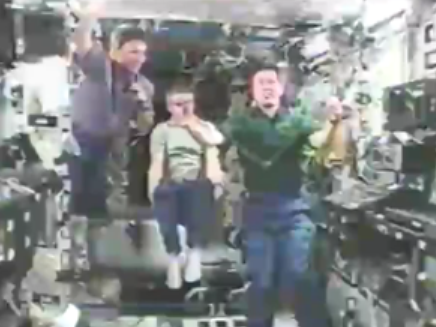
\includegraphics[scale=0.6]{T801.jpg} %中括号中的参数是设置图片充满文档的大小,你也可以使用小数来缩小图片的尺寸。
		%\caption{狼伴归途} %caption是用来给图片加上图题的
		%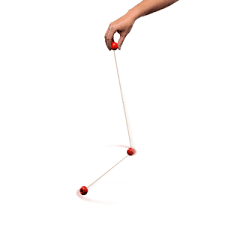
\includegraphics[scale=0.5]{T0102.png}
		%\label{wolf} %这是添加标签,方便在文章中引用图片。
	\end{figure}%figure环境\\
\\
	\indent Astrojax作为一个非线性系统,有无穷多种稳定模式,可以理解为:一个耗散系统中的受迫运动
	,对应模型是受迫谐振子。
	摩檫力是一种耗散,当输入功率等于输出功率时,以某种稳定的受迫振动频率运动。
	每一种玩法都对应了一种稳态,我们所寻找的稳态,其实就是一种稳定的受迫振动状态。
	
	加阻尼加驱动可能有稳定解,这种稳定解是什么呢?如何找到这种稳定解,利用同样的思路找到更多稳定解,从而为游戏带来更过花样!所以我们从弹簧振子讲起,再从单摆过渡到astrojax,最后分析分析一下我们的仿真模型原理.
	

	
	\section{弹簧振子}
	\subsection{简谐振动}
	%\centering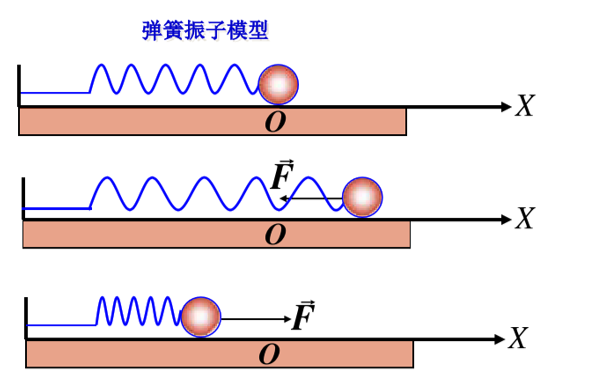
\includegraphics[scale=0.6]{T11.PNG}\\
	\begin{figure}[h] %figure环境,h默认参数是可以浮动,不是固定在当前位置。如果要不浮动,你就可以使用大写float宏包的H参数,固定图片在当前位置,禁止浮动。
		\centering %使图片居中显示
		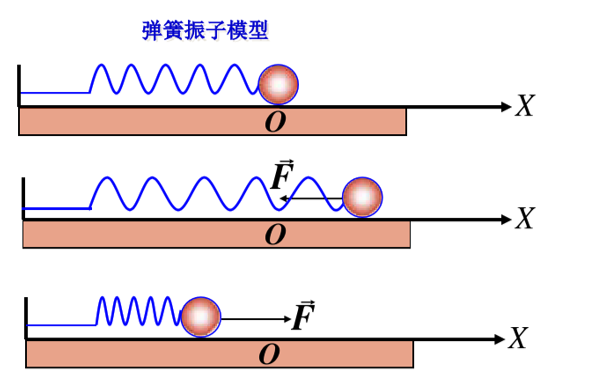
\includegraphics[scale=0.6]{T11.PNG} %中括号中的参数是设置图片充满文档的大小,你也可以使用小数来缩小图片的尺寸。
		%\caption{狼伴归途} %caption是用来给图片加上图题的
		%\label{wolf} %这是添加标签,方便在文章中引用图片。
	\end{figure}%figure环境
	\indent
	弹簧振子是研究简谐振动的一种理想模型,将光滑水平面物体(可视为质点)与一端固定的轻弹簧相连,就构成了一个弹簧振子。将物体在平衡位置不远处释放,物体将在回复力作用下返回平衡位置;由于惯性,物体将越过平衡位置,此后在回复力作用下减速,到达最大位移后返回,如此往复,形成在平衡位置的振动。
	%\noindent\textbf{}\
	
%	\centering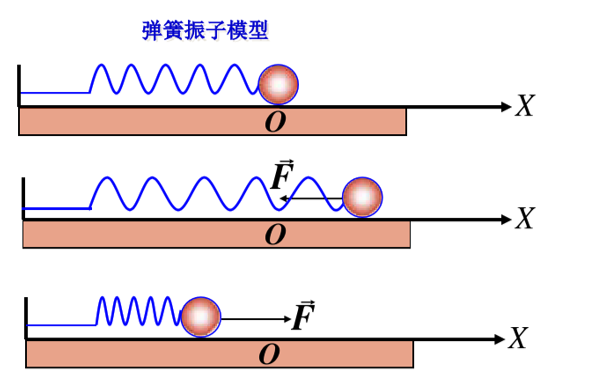
\includegraphics[scale=0.6]{T11.PNG}
	
	
	%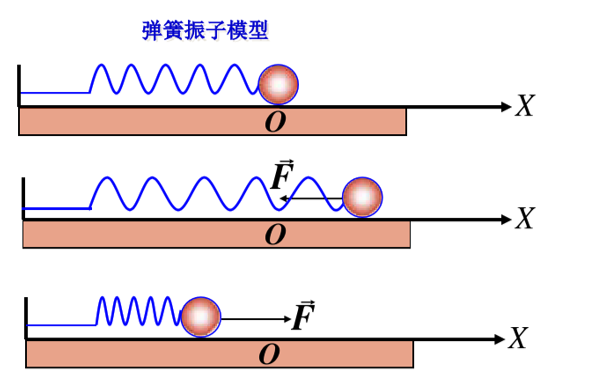
\includegraphics[scale=0.6]{T11.PNG}\
	
	
	%\noindent\textbf{}

	设物体质量为m,以O为坐标原点沿水平方向建立Ox坐标轴,当m在平衡位置附近发生不大的位移x时,作用在m上的弹性力可以表示为
	
	$$F=-kx$$
	
	式中k是弹簧的劲度系数,负号反映力的方向始终与位移方向相反,即指向平衡位置。这种与x成正比的回复力称为线性回复力。根据牛顿第二定律,可列出动力学方程为:
	
	$$m\frac{d^2x}{dt^2}=-kx$$
	
	令$\omega^2=\frac{k}{m}$,则上面的方程可以改写为
	
	$$\frac{d^2 x}{dt^2}+\omega^2 x =0$$
	
	这是一个二阶线性齐次微分方程,其解可以表示为
	
	$$x=Acos(\omega t+\phi) \qquad(1) $$
	
	式中A、φ为两个积分常量,ω则由系统自身特性决定。可见弹簧振子做简谐运动.
	对公式(1)两边对时间t求一阶和二阶导数,分别得到速度v和加速度a,即
	
	$$v=\frac{dx}{dt}=-A\omega sin(\omega t+\phi)$$
%	\clearpage
	%\thispagestyle{empty}
	$$a=\frac{d^2x}{dt^2}=-A\omega cos(\omega t+\phi)$$
	
	可见他们也做简谐振动可见他们也做简谐振动。
	
	\subsection{阻尼振动}
	%\begin{minipage}[b]{0.65\linewidth}
		\indent
		前面讨论的弹簧振子简谐振动,是既无外界输入能量,也无阻力存在从而没有能量耗散的理想振动,所以振动系统的能量守恒,振幅不会随时间发生变化,这样的振动称为无阻尼自由振动,然而任何实际振动过程都不可能没有能量损耗,例如弹簧振子的空气阻力和摩擦力、振荡电路的电阻等,它们都会使振动能量转化为热能:此外,振动还会以波的形式向四周辐射能量.所以,如无其他能量补充,系统的振幅和能量都会逐渐衰减,直至最后停止.这种系统在某种阻碍作用下,造成能量损失而使振幅随时间衰减的振动称为阻尼振动。\\
		
	%\end{minipage}
	%\hfill
	%\begin{minipage}[b]{0.35\linewidth}
%		\centering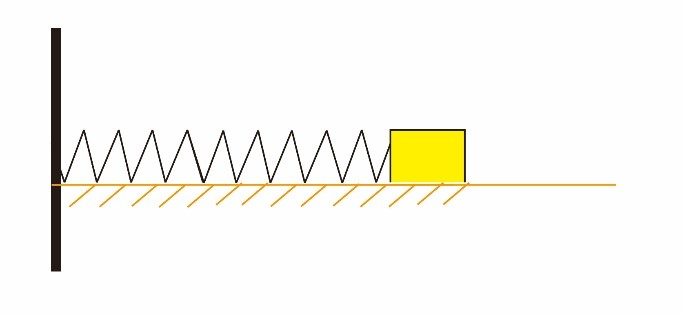
\includegraphics[height=8\baselineskip]{T12.jpg}
\begin{figure}[h] %figure环境,h默认参数是可以浮动,不是固定在当前位置。如果要不浮动,你就可以使用大写float宏包的H参数,固定图片在当前位置,禁止浮动。
	\centering %使图片居中显示
	\centering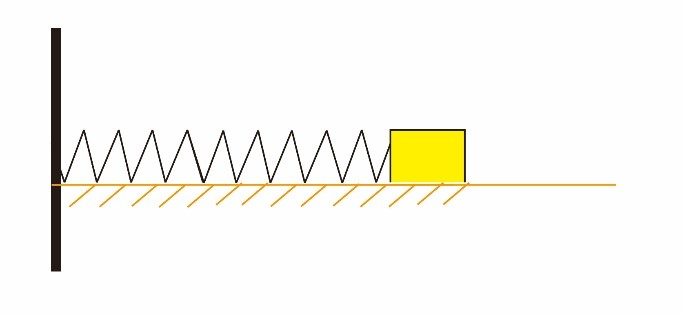
\includegraphics[height=8\baselineskip]{T12.jpg} %中括号中的参数是设置图片充满文档的大小,你也可以使用小数来缩小图片的尺寸。
	%\caption{狼伴归途} %caption是用来给图片加上图题的
	%\label{wolf} %这是添加标签,方便在文章中引用图片。
\end{figure}%figure环境
	%\end{minipage}
	机械振动中阻尼以黏性阻力为主,而电磁振荡中辐射引起的阻尼常常与黏性阻力相似.因此,下面仅考虑黏性阻力,在运动速率不大时,物体所受粘性阻力F可以认为与速率成正比,其方向与速度方向相反,即
	
	$$F_f=-\gamma\frac{dx}{dt}$$
	
	式中γ称为阻力系数,考虑黏性阻力后,水平弹簧振子的运动方程变为
	
	$$m\frac{d^2x}{dt^2}=-kx-\gamma\frac{dx}{dt}$$
	
	或
	
	$$\frac{d^2 x}{dt^2}+2\beta\frac{dx}{dt}+\omega^2 x=0  \qquad(2)$$
	
	式中$\omega= \sqrt{\frac{k}{m}}$是振动系统无阻尼时的固有角频率,$\beta=\frac{\gamma}{2m}$是表征系统阻尼大小的常量,称为阻尼系数。该微分方程特征值有两个,分别为
	
	$$\lambda=-\beta \pm\sqrt{\beta^2+\omega_0^2}$$
	
	按β大小不同,方程(1)的三种不同形式的解对应阻尼振动的三种可能的运动方式(如下图)
%	\clearpage
	%\thispagestyle{empty}
	%\textbf{}\
	
	
	
%	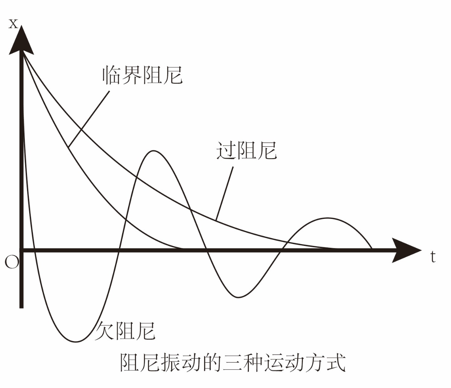
\includegraphics[scale=0.6]{T14.PNG}\
	
\begin{figure}[h] %figure环境,h默认参数是可以浮动,不是固定在当前位置。如果要不浮动,你就可以使用大写float宏包的H参数,固定图片在当前位置,禁止浮动。
	\centering %使图片居中显示
	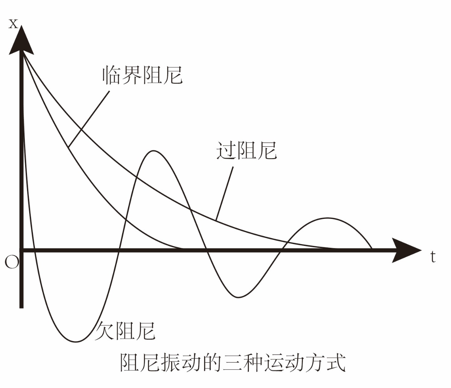
\includegraphics[scale=0.6]{T14.PNG} %中括号中的参数是设置图片充满文档的大小,你也可以使用小数来缩小图片的尺寸。
	%\caption{狼伴归途} %caption是用来给图片加上图题的
	%\label{wolf} %这是添加标签,方便在文章中引用图片。
\end{figure}%figure环境	
	
	\noindent\textbf{以下对三种情况分别讨论}
	\subsubsection{欠阻尼运动}
	当阻尼较小,即当$\beta^2<\omega^2$时,方程(2)的解为
	$$x=A_0e^{-\beta t}cos(\omega t+\phi)$$
	
	可见系统的振幅不断衰减,所以不是简谐报动,但仍然在平衡位置附近作往复运动,可以看作是一种准周期运动。常称为欠阻尼振动.式中
	
	$$\omega=\sqrt{\omega_0^2-\beta^2}<\omega_0$$
	
	可见,与无阻尼自由振动相比,由于阻尼存在,其“频率”变小,而“周期”则变长,为
	
	$$T=\frac{2\pi}{\omega}=\frac{2\pi}{\sqrt{\omega_0^2-\beta^2}>\frac{2\pi}{\omega}}$$
	
	振幅衰减的快慢程度,可用相邻两次振动的振幅之比的对数来反映,称为对数减缩率,用$\Lambda$表示,即
	
	$$T=\frac{2\pi}{\omega}=\frac{2\pi}{\sqrt{\omega_0^2-\beta^2}}>\frac{2\pi}{\omega}$$
	
	可见Λ与β成正比。
	\subsubsection{过阻尼运动}
	当阻尼较大,即当$\beta^2>\omega^2$时,方程(2) 的解为
	$$x=c_1e^{-(\beta-\sqrt{\beta^2-\omega_0^2})t}+c_2e^{-(\beta+\sqrt{\beta^2-\omega_0^2})t}$$
	
	这不是一种周期运动,物体将缓慢的逼近平衡位置,但不会越过平衡位置,即称为过阻尼振动。
	\subsubsection{临界阻尼振动}
	当$\beta^2=\omega^2$时,方程(2)的解为
	%	\clearpage
%	\thispagestyle{empty}
	$$x=(c_1+c_2t)e^{-\beta t}$$

	这是一种刚好介于欠阻尼振动和过阻尼之间的临界情况,称为临界阻尼。
	和前两种情况相比,这种非周期性运动能够在最短时间回到平衡位置并停止下来,因此要让物体在不发生振动的情况下最快回到平衡位置,常用施加临界阻尼的方法。例如指针式仪表中常使仪表工作在临界阻尼状态,这样指针可以快速地停在读数值处.
	\subsection{受迫振动}	
	
	
	\begin{figure}[h] %figure环境,h默认参数是可以浮动,不是固定在当前位置。如果要不浮动,你就可以使用大写float宏包的H参数,固定图片在当前位置,禁止浮动。
		\centering %使图片居中显示
		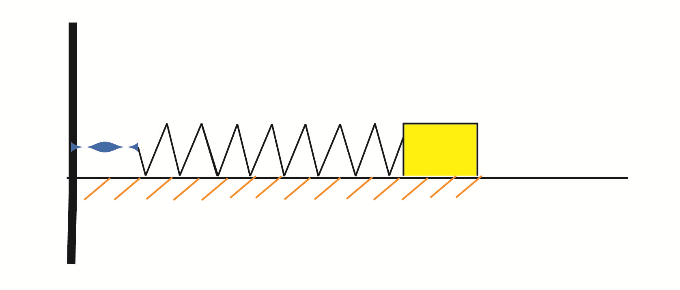
\includegraphics[height=8\baselineskip]{T15.png}%中括号中的参数是设置图片充满文档的大小,你也可以使用小数来缩小图片的尺寸。
		%\caption{狼伴归途} %caption是用来给图片加上图题的
		%\label{wolf} %这是添加标签,方便在文章中引用图片。
	\end{figure}%figure环境	
	%\begin{minipage}[b]{0.55\linewidth}

		在有阻尼的情况下,由于能量损耗,系统最终会停止在平衡位置,要使系统的振动状态持久而不衰减,可以对系统施加一个周期性的外界驱动力,通过做功不断向系统提供能量来实现,这种在周期性外界驱动力作用下的振动,称为受迫振动
%	\end{minipage}
	\hfill
%	\begin{minipage}[b]{0.45\linewidth}
%		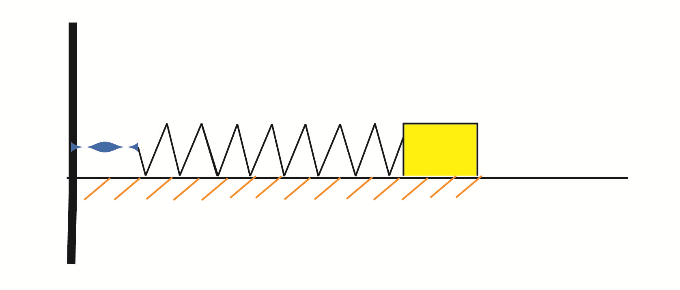
\includegraphics[height=8\baselineskip]{T15.png}
%	\end{minipage}

	设系统受到的简谐驱动力为F=cosωft的作用,F是力幅,$\omega_f$是驱动力变化的角频率,则受迫振动的微分方程
	$$m\frac{d^2x}{dt^2}+\gamma\frac{dx}{dt}+kt=Fcos(\omega_f t)$$
	
	或者
	
	$$\frac{d^2x}{dt^2}+2\beta\frac{dx}{dt}+\omega_0^2t=f_0cos(\omega_f t)$$
	
	该微分方程的解为:
	
	$$x=A_0e^{-\beta t}cos(\omega t+\phi)+Acos(\omega_f t+\phi) \qquad(3)$$
	
	其中第二项为一种稳定的等幅振动,它表示阻尼振动衰减后系统在简谐外力作用下受迫振动的稳定状态,成为稳态响应
	
	$$x=Acos(\omega t+\phi)\qquad (4)$$
	
	将该解带入(3),容易得到
	
	$$A=\frac{f_0}{\sqrt{(\omega_0^2-\omega_f^2)^2+4\beta^2\omega_f^2}}$$
	
	$$tan(\phi)=-\frac{2\beta \omega_f}{\omega_0^2-\omega_f^2}$$
	
	4)式表示的稳定受迫振动状态,形式上虽与简谐振动类似,但它不是简谐振动,因为它的频率为外力频率ωf.与固有频率ω0无关.振幅A和φ也
%	\clearpage
%	\thispagestyle{empty}
	\noindent 并非取决于初始条件,而是与系统、阻尼和外界驱动力的特征有关。可见,系统在无阻尼也没有外界作用,即在线性回复力作用下的无阻尼自由振动才是简谐振动,筒谐振动的频率仅由系统性质决定。
	
	
	\subsection{共振}
	稳定受迫振动的频率虽与外力相同,但相位却不一样,由于阻尼的存在,使得振动对外里的响应滞后,相位上落后了$\phi$,根据受迫振动的方程解可得知,当外界驱动力的频率为某一特定值时,受迫振动中位移振幅将达到极大值,这一现象称为位移共振,称为共振。
	共振时对应的$\omega_f$值为$\omega_t$,称为共振角频率。由极值条件$\frac{dA}{d\omega_f}=0$,可以求得$\omega_f$和共振时的振幅At分别为
	
	$$\omega_f=\sqrt{\omega^2-2\beta^2}$$,$$A=\frac{f_0}{2\beta\sqrt{\omega_0^2-2\beta^2}}$$
	
	
	下图所示是不同阻尼情况下A随外界驱动力的角频率变化的曲线ωf。由此看出一般共振频率不等于系统的固有频率,阻尼β越小,则共振频率越接近于固有角频率$\omega_0$,Ar也越大,当$\beta<<\omega_r$
	时,共振频率$\omega_0\approx \omega_0$,共振振幅趋于无穷大.
	\textbf{}\
	
	
	
	%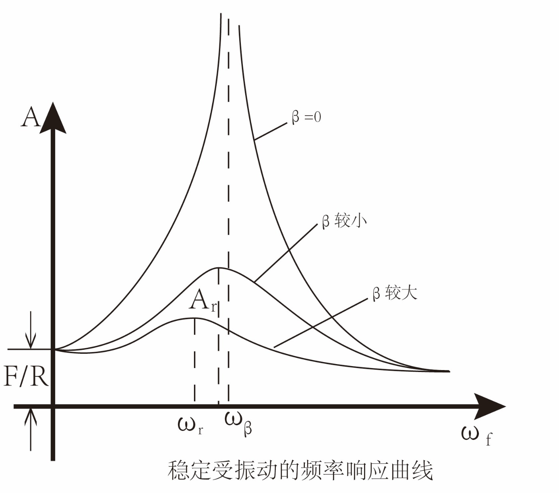
\includegraphics[scale=0.6]{T16.PNG}\
	
	\begin{figure}[h] %figure环境,h默认参数是可以浮动,不是固定在当前位置。如果要不浮动,你就可以使用大写float宏包的H参数,固定图片在当前位置,禁止浮动。
		\centering %使图片居中显示
		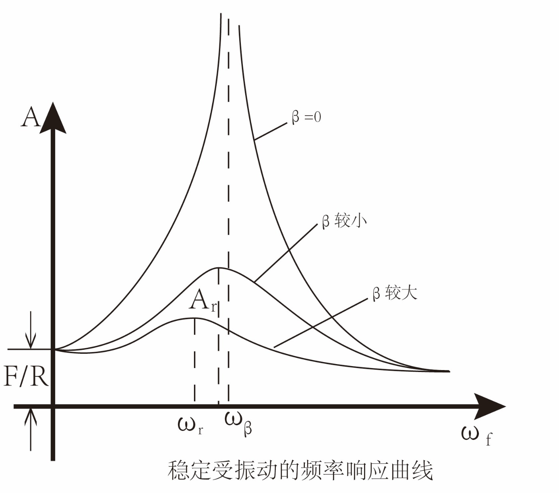
\includegraphics[scale=0.6]{T16.PNG} %中括号中的参数是设置图片充满文档的大小,你也可以使用小数来缩小图片的尺寸。
		%\caption{狼伴归途} %caption是用来给图片加上图题的
		%\label{wolf} %这是添加标签,方便在文章中引用图片。
	\end{figure}%figure环境	
	
	\noindent\textbf{}
	
	对受迫振动解对时间求导数可得速度振幅为
	
	$$v_m=\omega_fA+\frac{\omega_f f_0}{\sqrt{\omega_0^2-\omega_f^2}+4\beta^2\omega_f^2}$$
	
	
	当$\omega_f=\omega_0$时速度振幅最大,为$\frac{f}{2\beta}$,这称为速度共振。速度共振时振动位移的相位比驱动力落后$\frac{\pi}{2}$,即振动速度与驱动力同相位,因此驱动力总是做正功,从而外界把能量转化为系统能量,因此速度共振也称为能量共振。一般情况下,由于位移共振与速度共振频率不同,位移共振时驱动力并非
	%\clearpage
	%\thispagestyle{empty}
	\noindent 总是做正功。但在阻尼$\beta$趋近于零的情况下,当$\omega_r=\omega_0$时位移共振和速度共振同时发生,使位移振幅和速度振幅急剧增大,系统则发生强烈共振。
	
	
	
	
	
	
	
	
	
	\section{单摆}
	%\begin{minipage}[b]{0.65\linewidth}
		单摆是能够产生往复摆动的一种装置,将无重细杆或不可伸长的细柔绳一端悬于重力场内一定点,另一端固结一个重小球,就构成单摆。
		若小球只限于铅直平面内摆动,则为平面单摆,若小球摆动不限于铅直平面,则为球面单摆。
		
		
	%\end{minipage}
	\hfill
	%\begin{minipage}[b]{0.35\linewidth}
	%	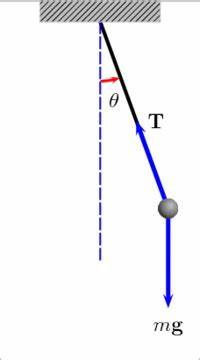
\includegraphics[height=8\baselineskip]{T41.PNG}
	%\end{minipage}
	
	
	\begin{figure}[h] %figure环境,h默认参数是可以浮动,不是固定在当前位置。如果要不浮动,你就可以使用大写float宏包的H参数,固定图片在当前位置,禁止浮动。
		\centering %使图片居中显示
		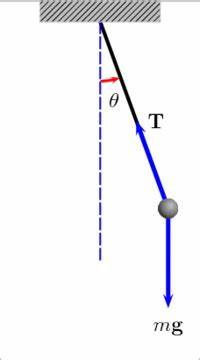
\includegraphics[height=8\baselineskip]{T41.PNG} %中括号中的参数是设置图片充满文档的大小,你也可以使用小数来缩小图片的尺寸。
		%\caption{狼伴归途} %caption是用来给图片加上图题的
		%\label{wolf} %这是添加标签,方便在文章中引用图片。
	\end{figure}%figure环境	


	\subsection{球面单摆的圆周运动(无阻尼)}
	%\begin{minipage}[b]{0.65\linewidth}
		球的运动轨迹为圆周,圆周半径为  $L sin(\theta)$          ,可列出如下方程:
		
		$$mg tan(\theta)=m\omega^2Lsin(\theta)$$
		
		当极角给定时,我们可以求得其稳定运动时的角速度和半径:
		
		$$R=Lsin(\theta)$$
		
		$$\omega=\sqrt{\frac{1}{Lcos(\theta)}}$$
%	\end{minipage}
	\hfill
	%\begin{minipage}[b]{0.35\linewidth}
		%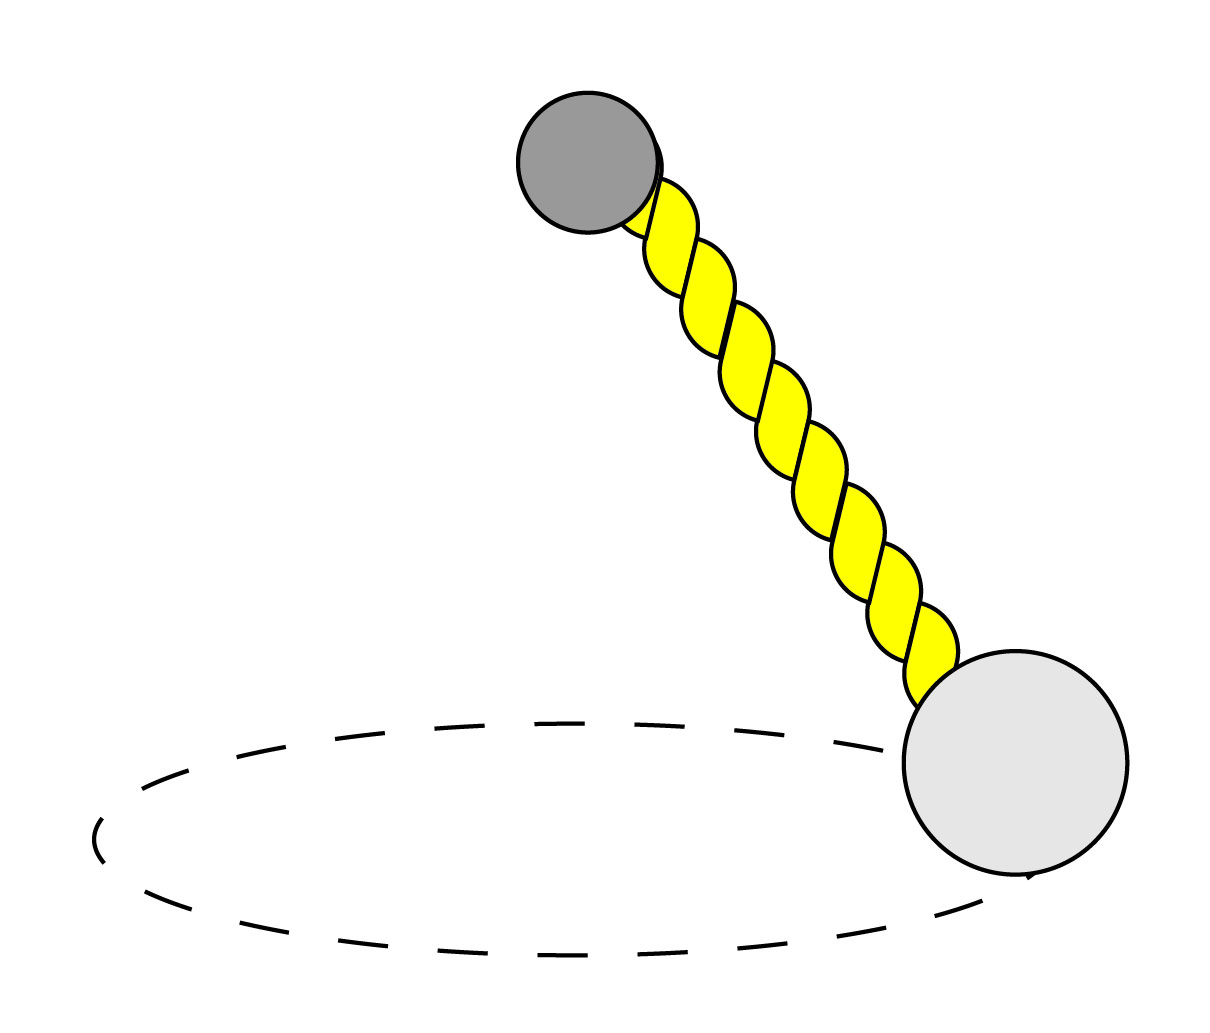
\includegraphics[height=8\baselineskip]{T42.jpg}
	%\end{minipage}
	\begin{figure}[h] %figure环境,h默认参数是可以浮动,不是固定在当前位置。如果要不浮动,你就可以使用大写float宏包的H参数,固定图片在当前位置,禁止浮动。
	\centering %使图片居中显示
	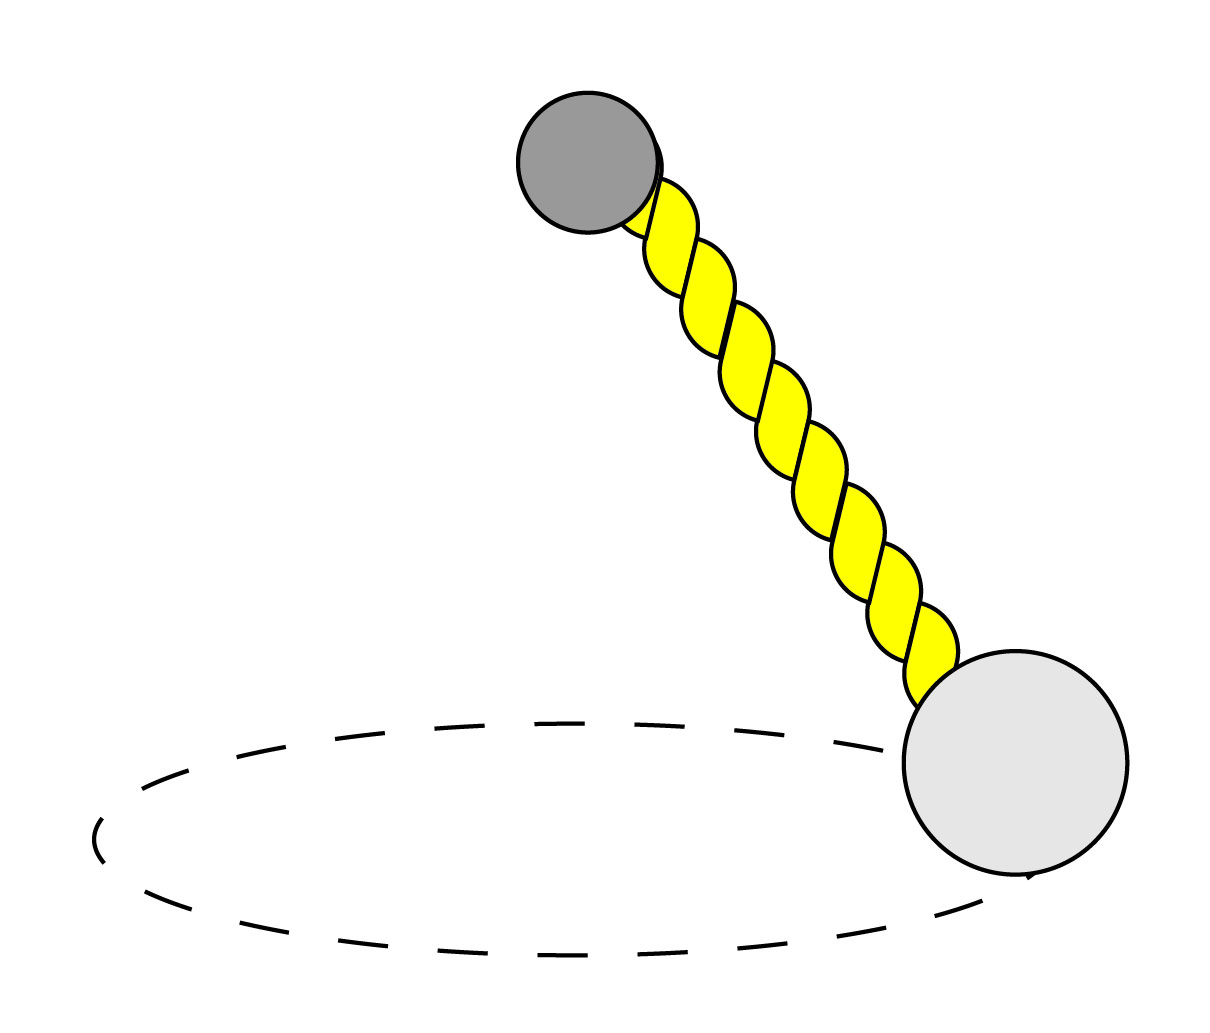
\includegraphics[height=8\baselineskip]{T42.jpg} %中括号中的参数是设置图片充满文档的大小,你也可以使用小数来缩小图片的尺寸。
	%\caption{狼伴归途} %caption是用来给图片加上图题的
	%\label{wolf} %这是添加标签,方便在文章中引用图片。
\end{figure}%figure环境	

	\subsection{球面单摆的圆周运动有阻尼}
	当考虑阻尼时,假设阻力的大小与小球的速度大小成正比,方向与小球的运动速度方向相反,从而得出一下方程:
	$$\frac{dv}{dt}=-\eta v$$
	
	$$m\frac{v^2}{Lsin(\theta)}=mgtan(\theta)$$
	\begin{figure}[h] %figure环境,h默认参数是可以浮动,不是固定在当前位置。如果要不浮动,你就可以使用大写float宏包的H参数,固定图片在当前位置,禁止浮动。
	\centering %使图片居中显示
	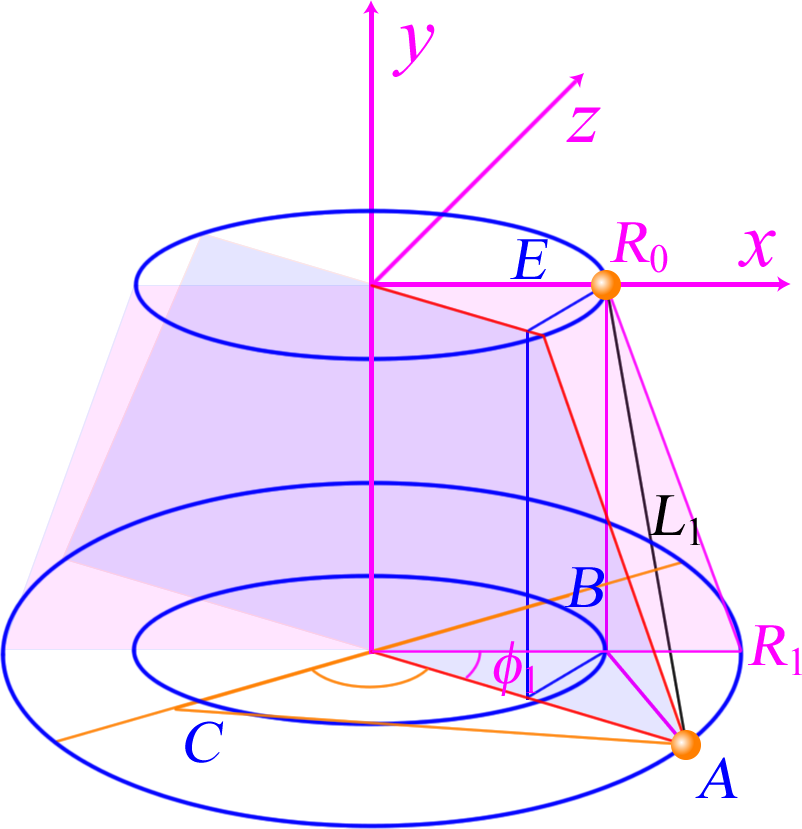
\includegraphics[height=16\baselineskip]{T800.png} %中括号中的参数是设置图片充满文档的大小,你也可以使用小数来缩小图片的尺寸。
	%\caption{狼伴归途} %caption是用来给图片加上图题的
	%\label{wolf} %这是添加标签,方便在文章中引用图片。
\end{figure}%figure环境	
	
	
	
	
%	\clearpage
%	\thispagestyle{empty}
	\subsection{球面单摆的圆周运动(受迫运动)}
	\begin{minipage}[b]{0.65\linewidth}
		对于有阻尼球面摆而言,$R_1,\phi_1,h_1$是已知的,
		$$T_{01||}=\eta \omega R_1$$
		
		$$t_{01\perp}=m_1 \omega^2 R_1$$
		
		$$T_{01y}=m_1g$$
		
		绳长约束$$L_1^2=R_0^2+R_1^2-2R_0R_1cos(\phi)+H_1^2$$
		
		受力方向约束
		
		$$\frac{T_{01y}}{\sqrt{T_{01||}^2+t_{01\perp}^2}}=\frac{H_1}{\sqrt{L_1^2=R_0^2+R_1^2-2R_0R_1cos(\phi)}}$$
		
		受力方向约束
		$$\frac{T_{01||}}{t_{01\perp}}=tan(\pi-\alpha_1)=\frac{sin(\phi)}{\frac{R_1}{R_0}-cos(\phi)}$$
	\end{minipage}
	\hfill
	\begin{minipage}[b]{0.35\linewidth}
		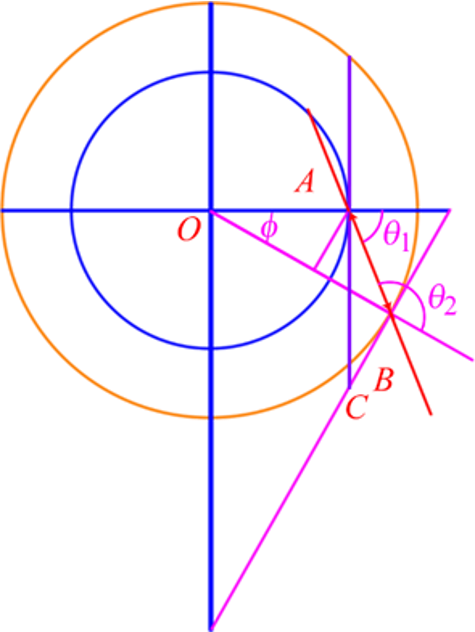
\includegraphics[height=8\baselineskip]{T44.png}
	\end{minipage}
	\section{Astrojax}
	\subsection{1.Astrojax——复杂的双摆球运动}
	\begin{minipage}[b]{0.65\linewidth}
		还记得曾经风靡一时的悠悠球吗,它已经逐渐被人们所遗忘,不过目前却出现了一个类似的替代品,悠悠球是一根绳,一个球的花式运动,从1A到5A玩法多种多样。最近国际上新出现的类似的产品由三个球一根绳组成,一个球在最上端,有人来控制,一个球在最下端,另一个在中间。它就是astrojax,如图所示。一个新兴的悠悠球,它也有许多种玩法,比如horizontal orbits, vertical orbits, butterfly orbits, or wild and crazy patterns。这些不过是开始而已。
	\end{minipage}
	\hfill
	\begin{minipage}[b]{0.35\linewidth}
		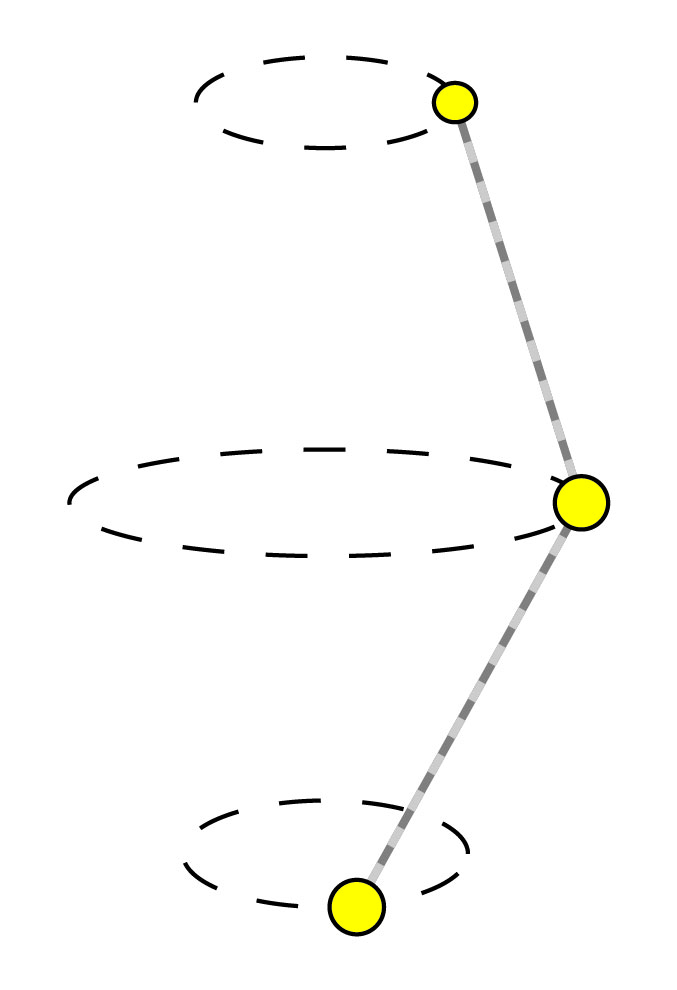
\includegraphics[height=8\baselineskip]{T01.jpg}
	\end{minipage}
	这项运动,已经有许多人在参与了,玩法更是多种多样,它的兴起得益于NASA宇航员在太空表演的一段视频,于是越来越多的人发现了它的存在。Astrojax是一款风靡全美国的玩具:将绳子穿过一个带有洞的球,这样球就可以沿着绳子自由移动。把另一个球系在绳子的一端。当你周期性地移动绳子的自由端时,你可以观察到两个球的复杂运动。此系统不同于双摆---中间的球可以沿着绳子自由滑动。因其运动类似于行星,故命名为Astrojax。更是有许多能人义士开发了多种多样的应用领域。最简单的像
	%\clearpage
	%\thispagestyle{empty}
	是,舞台表演这一类的玩法,进一步还有医学领域的物理疗法帮助病人们做康复训练,更深层次的,就是专业球手的手眼协调高难度花式动作。除此之外,这样有趣的玩具怎么可能不引起科学家们的重视呢,各个物理方面的科学家们对这一现象展开了多种多样的研究,能量,摆动,周期等一系列话题,今天,我们就稳定状态也展开一次对玩具的研究,实现在电脑上玩新玩具。
	\subsection{水平轨道无阻尼运动}
	\subsubsection{模型建立}
	\begin{minipage}[b]{0.65\linewidth}
		首先,让我们来看一下它在水平轨道的无阻尼运动,这是astrojax的最简单的玩法之一,也是最简单的稳定状态,仔细看一下这一运动状态。最上端有一个质量为m0的小球,中间有一个m1的不固定小球在轨道中间可以自由旋转,最下端是一个质量为m2的小球,跟随上面的小球一起做圆周运动。那么这样问题就很清楚了,就是如右图所示的简单模型。
	\end{minipage}
	\hfill
	\begin{minipage}[b]{0.35\linewidth}
		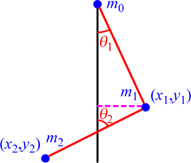
\includegraphics[height=8\baselineskip]{T02.png}
	\end{minipage}
	\subsubsection{方程求解}
	可以发现这里一共有六个未知量T球的圆周运动周期, $\omega$圆周运动的角频率, $\theta_1$上方两个球连线与竖直方向的夹角,  $\theta_2$下方两个小球与竖直方向的夹角, L1第一段绳子的长度, L2后半段绳子的长度,同时还有五个方程,
	$$T\cos{\theta_1}=m_1g+T\cos{\theta_2}$$
	
	$$T\sin{\theta_1}+T\sin{\theta_2}=m_1\omega^2l_1\sin{\theta_1}$$
	
	$$T\sin{\theta_2}=m_2\omega^2(l_2\sin{\theta_2-l_1\sin{\theta_1)}}$$
	
	$$T\cos{\theta_2}=m_2g$$
	
	$$l_1+l_2=l_0$$
	
	这样的话,只要我们给定了其中任何一个未知量,那么剩下的未知量就都是可解的了,因此,这样的运动状态就是可以完全确定下来的了。那么,这就是我们通过计算机模拟仿真实现的第一个图景。
	\clearpage
	\thispagestyle{empty}
	\subsubsection{问题拓展}
	同时就这个问题我们还做了一些与实际相关的问题的探讨,我们通过上面这些方程得出的数值解,输入到计算机中进行数据的解析,得到了astrojax在无阻尼驱动状态下,达到稳定状态后能量随着极角的变化,以及中间球和底端球的坐标随时间的变化。
		\begin{figure}[htb]
		\centering
		{
			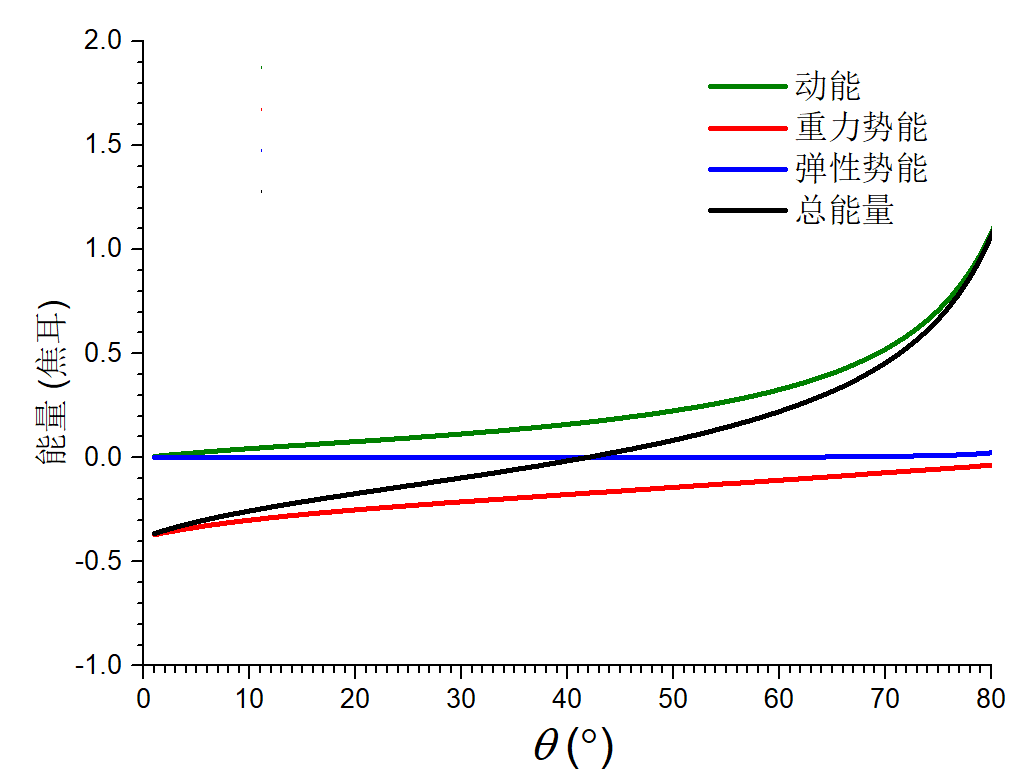
\includegraphics[width=6cm]{T04.png}}
		\hspace{0in}   
		{
			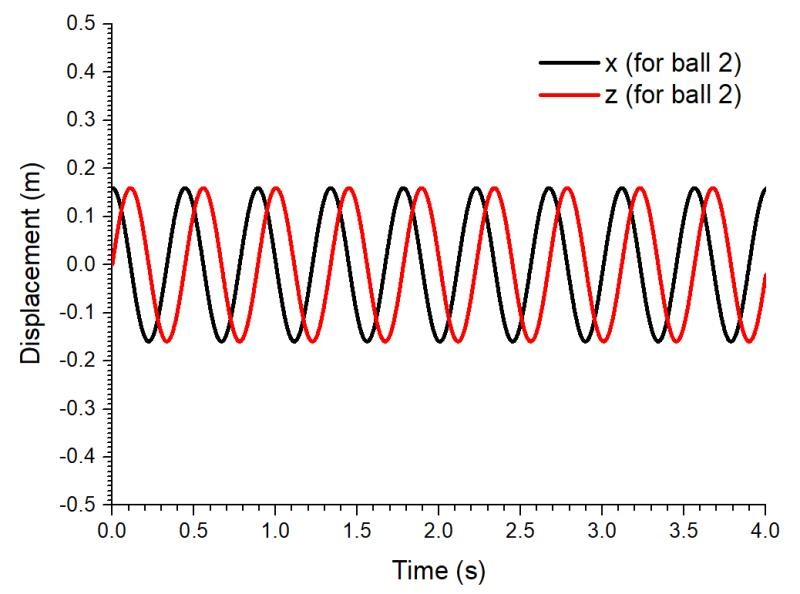
\includegraphics[width=6cm]{T05.jpg}}
		\hspace{0in}
		{
			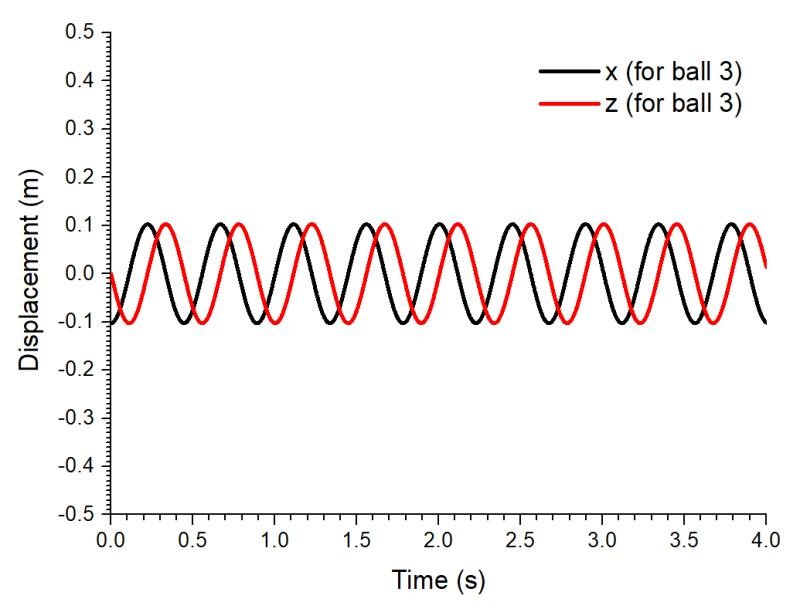
\includegraphics[width=7cm]{T06.jpg}}
		\hspace{0in}
		
	\end{figure}
	
	\subsection{水平轨道受迫运动——基础招式}
	\subsubsection{模型建立}
	既然我们已经分析清楚了最基础的运动状态,那么就可以来看看实际的应用场景,astrojax既然是作为一项玩具运动项目在美国兴起的,那么它的最基础的招式就当然应该作为我们运动分析必不可少的一环,也就是,接下来我们应该看一看astrojax在水平运动的时候的具体运动过程的探讨.
	\clearpage
	\thispagestyle{empty}
	\begin{minipage}[b]{0.65\linewidth}
		我们可以将问题简化一下,将三个小球看作三个质点,将中间的小球记作A,将上面的小球记作B,最下面的小球记作C,并且假设他们在空间范围内做逆时针转动。既然我们已经将这样的实际模型放在了空间范围内进行研究,就应该应用一下最普遍的办法,空间直角坐标系,因为最后是要应用于unity3D进行虚拟仿真的模型建立,那么就可以直接应用unity3D的内置坐标系来建立对应的方程组。如右图所示。
	\end{minipage}
	\hfill
	\begin{minipage}[b]{0.35\linewidth}
		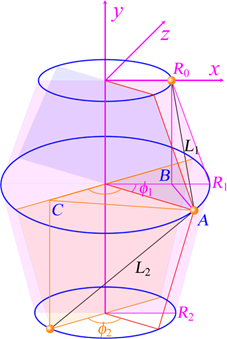
\includegraphics[height=8\baselineskip]{T07.png}
	\end{minipage}
	\subsubsection{方程求解}
	选取顶端的小球做圆周运动的圆心作为空间直角坐标系的原点,水平向右为x轴,水平向后的z轴,以及竖直向上的y轴,建立左手坐标系,那么,xyz三个方向的单位向量就是
	
	$\vec{x}=(1,0,0)'$
	
	$\vec{y}=(0,1,0)'$
	
	$\vec{z}=(0,0,1)'$
	
	可以假设顶端小球半径为R0,中间小球半径为R1,底端小球半径为R2,顶端小球与中间小球的绳子长度为L1,中间小球与底端小球的绳子长度为L2,第一个小球所在位置投影到第二个小球圆周运动的平面,那么两条线的夹角记作Φ1,这就是这两个小球做圆周运动时对应的相位差,同理,第二个小球投影到底端小球,这两个小球的相位差记作Φ2,于是得到B、A、C三个小球的对应坐标位置。
	
	$B:((R_0\cos{(\omega t)}),0,R_0\sin{(\omega t)})$
	
	$A:(R_1\cos{(\omega t-\phi_1)},-h_1,R_0\sin{(\omega t-\phi_1)})$
	
	$C:(R_2\cos{(\omega t-\phi_1-\phi_2)},-h_1-h_2,R_0\sin{(\omega t-\phi_1-\phi_2)})$
	
	由此就可以得到AB和CA向量的坐标表示,因此得到相应的单位向量的坐标表示。
	
	$\vec{AB}=(R_0\cos{(\omega t)}-R_1\cos{(\omega t-\phi_1)},h_1,R_0\sin{(\omega t)}-R_0\sin{(\omega t-\phi_1)})$
	
	$\vec{CA}=(R_1\cos{(\omega t-\phi_1)}-R_2\cos{(\omega t-\phi_1\phi_2)},h_2,R_0\sin{(\omega t-\phi_1)}-R_0\sin{(\omega t-\phi_1-\phi_2)})$
	\clearpage
	\thispagestyle{empty}
	$\vec{e_1}=\frac{\vec{AB}}{\vert\vec{AB}\vert}$

	$\vec{e_2}=\frac{\vec{CA}}{\vert\vec{CA}\vert}$
	
	从上往下俯视观察,得到对应的平面投影,
		\textbf{}\
	
	
	
%	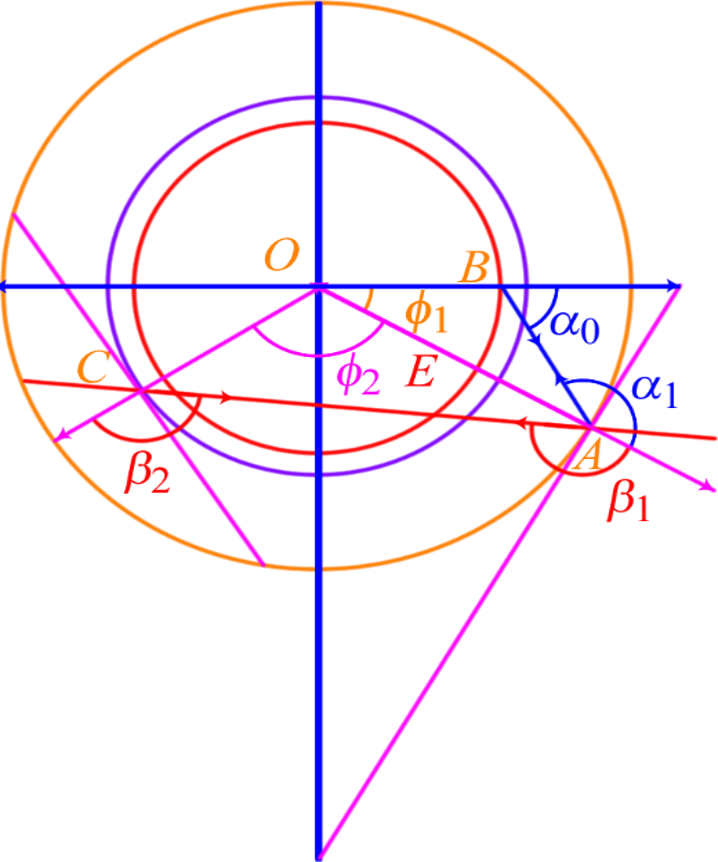
\includegraphics[scale=0.4]{T08.PNG}\
	
	\begin{figure}[h] %figure环境,h默认参数是可以浮动,不是固定在当前位置。如果要不浮动,你就可以使用大写float宏包的H参数,固定图片在当前位置,禁止浮动。
	\centering %使图片居中显示
	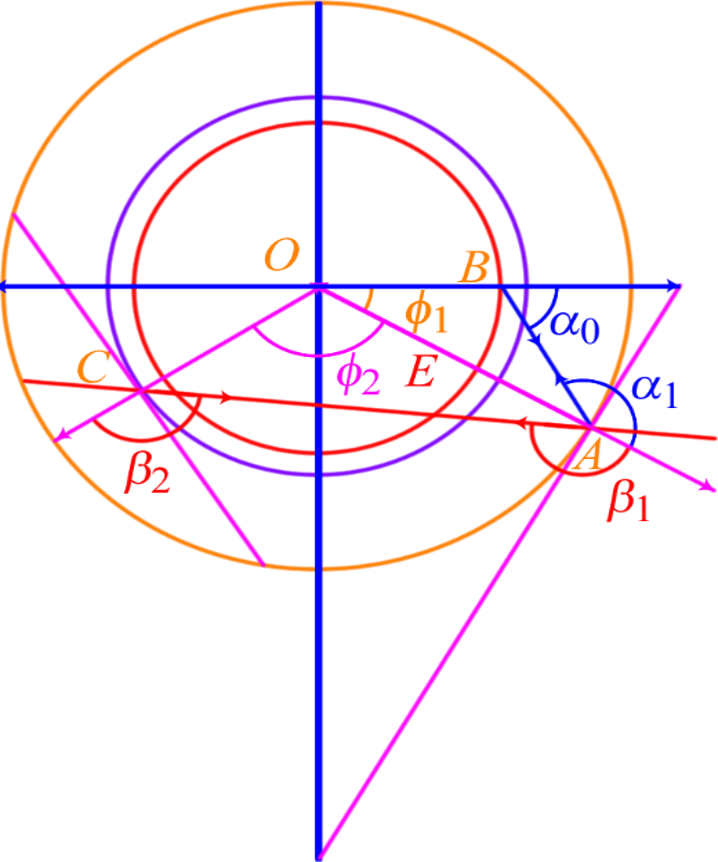
\includegraphics[scale=0.4]{T08.PNG} %中括号中的参数是设置图片充满文档的大小,你也可以使用小数来缩小图片的尺寸。
	%\caption{狼伴归途} %caption是用来给图片加上图题的
	%\label{wolf} %这是添加标签,方便在文章中引用图片。
\end{figure}%figure环境	
	
	\noindent\textbf{}
	
	这样的话问题就简化为在平面运动的圆周运动,这样的运动就不得不提到圆周运动最普遍的问题处理方法,将A和C分解为对应的切向加速度以及对应的轴向加速度,并且可以由此得到对应方向的单位向量。
	
	$\vec{A_{\perp}}=(-R_1\cos{(\omega t-\phi_1)},0,-R_1\sin{(\omega t-\phi_1)})$
	
	$\vec{C_{\perp}}=(-R_2\cos{(\omega t-\phi_1-\phi_2)},0,-R_2\sin{(\omega t-\phi_1-\phi_2)})$
	
	$\vec{e_{A\perp}}=\frac{\vec{A_{\perp}}}{\vert\vec{A_{\perp}}\vert}$
	
	$\vec{e_{C\perp}}=\frac{\vec{C_{\perp}}}{\vert\vec{C_{\perp}}\vert}$
	
	$\vec{A_{||}}=(-R_1\omega\sin{(\omega t-\phi_1)},0,R_1\omega\cos{(\omega t-\phi_1)})$
	
	$\vec{C_{||}}=(-R_2\omega\sin{(\omega t-\phi_1-\phi_2)},0,-R_2\omega\cos{(\omega t-\phi_1-\phi_2)})$
	
	$\vec{e_{A||}}=\frac{\vec{A_{||}}}{\vert\vec{A_{||}}\vert}$
	
	$\vec{e_{C||}}=\frac{\vec{C_{||}}}{\vert\vec{C_{||}}\vert}$
	
	当我们建立了这些基础向量,对于这个实际难题就可以直接简化为最简单的图景。
	因为对于astrojax来说中间小球是要自由滑动的,因此可以忽略掉它与绳子之间的摩擦阻力,那么,对于中间小球就可以简化为动滑轮,这样的话,绳子两端就可以近似处理为两端相等的绳子拉力,于是,将中间与底端小球看作一个整体,将上半段绳子投影到竖直方向,这个分力就应
	\clearpage
	\thispagestyle{empty}
	该与中间和底端的小球重力平衡,同样的,这段绳子投影到水平面内,这个分力就可以作为后两个小球做圆周运动的轴向力,驱动中间和底端小球做圆周运动。同理,对于后半段绳子做同样的投影处理,就可以都得到对于底端小球的受力分析。因此得到了这样的六个方程,
	
	$T\vec{e_1}·\vec{y}=(m_1+m_2)g$
	
	$T\vec{e_2}·\vec{y}=m_2g$
	
	$T\vec{e_1}·\vec{e_{A\perp}}-T\vec{e_2}·\vec{e_{A\perp}}=\omega^2m_1R_1$
	
	$T\vec{e_1}·\vec{e_{A||}}-T\vec{e_2}·\vec{e_{A||}}=\eta\omega R_1$
	
	$T\vec{e_2}·\vec{e_{C||}}=\eta\omega R_2$
	
	$T\vec{e_2}·\vec{e_{C\perp}}=\omega^2m_2R_2$
	
	这样的话,对于之前的六个未知量就都可解了。
	既然我们已经得到的这样的六个未知量,于是我们就可以通过如下公式
	\textbf{}\
	
	
	
	\includegraphics[scale=0.4]{T09.PNG}\
	
	
	
	\noindent\textbf{}
	\textbf{}\
	
	
	
	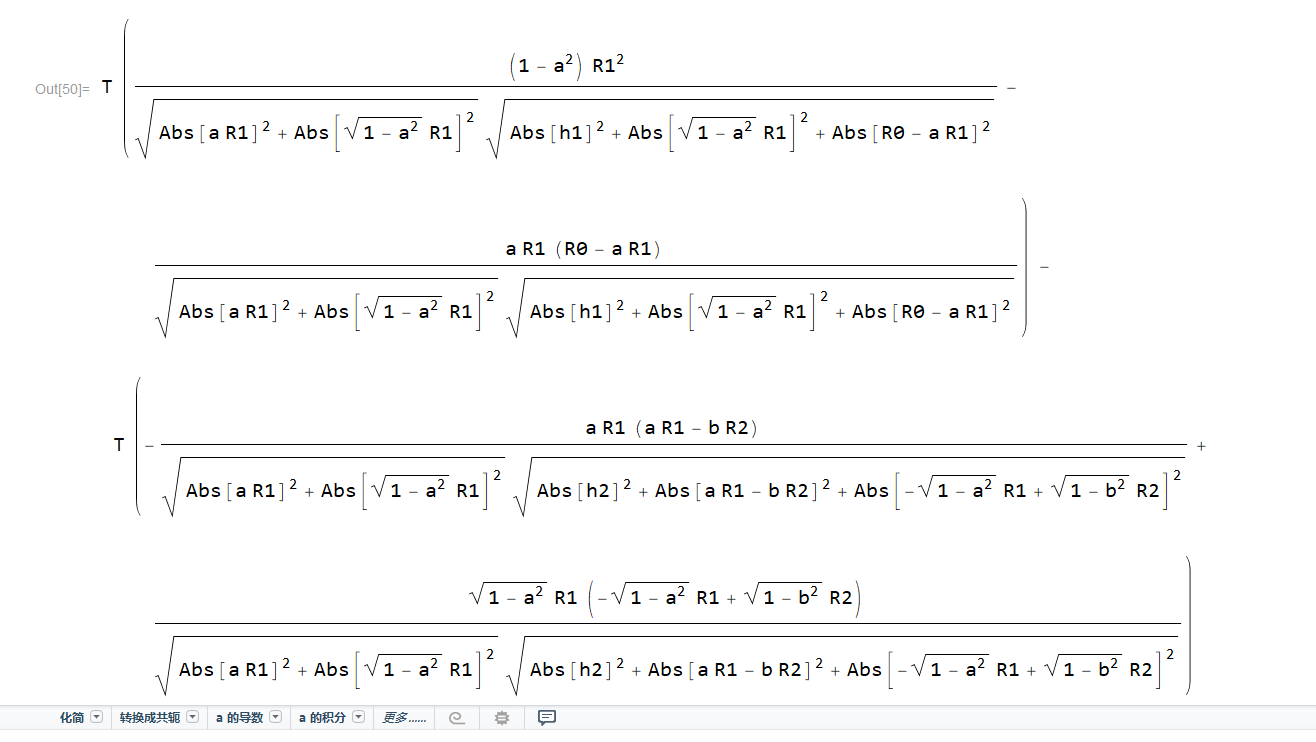
\includegraphics[scale=0.4]{T001.PNG}\
	
	
	
	\noindent\textbf{}


	\textbf{}\
	
	
	
	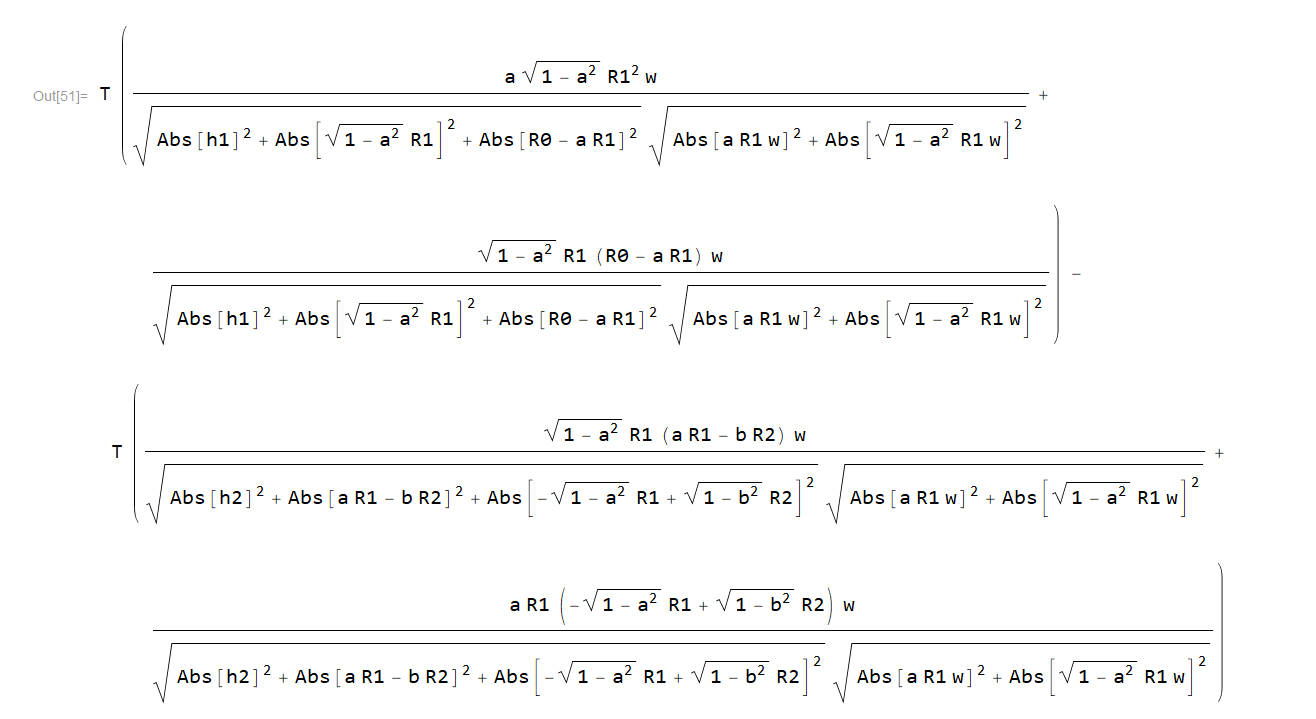
\includegraphics[scale=0.4]{T011.PNG}\
	
	
	
	\noindent\textbf{}
		\thispagestyle{empty}
	\textbf{}\
	
	
	
	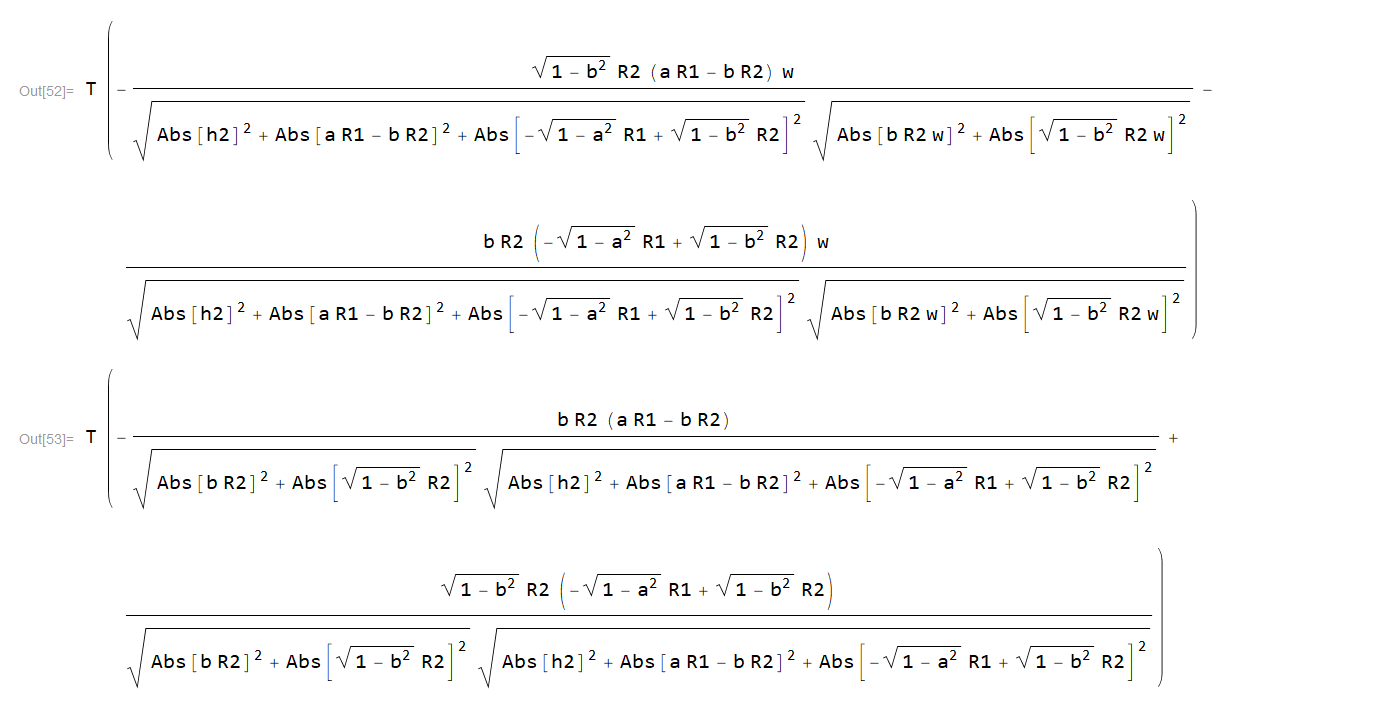
\includegraphics[scale=0.4]{T012.PNG}\
	
	
	
	\noindent\textbf{}
	计算得到相应的数值解,将这些得到的数值解带入到我们建立的虚拟仿真实验中就可以实现真正的在电脑上玩玩具。
	\clearpage
	\thispagestyle{empty}
	
	
	\section{仿真算法分析}
	\subsection{保辛算法}
	
		因为哈密顿系统的的正则方程在辛变换下形式不变,辛算法是基于哈密顿力学的基本原理而提出的保哈密顿系统的差分法,它使离散化后的差分方程保持原有的系统的辛结构,因此辛算法具有长时间的稳定性。
	
		一般的算法,误差(步长以及计算机字长造成)会随步数指数增加。减小步长会造成迭代次 数的增加。如果保证在积分
	每一步都作辛变换,则可以显著控制误差的积累。
	\subsection{蛙跳法具体应用}
	根据每一时刻的位置矢量,动量来计算该时刻的受力,求得其加速度,速度,利用“蛙跳法“解微分方程求其位置变化;
	\noindent\textbf{}\
	
	
	
%	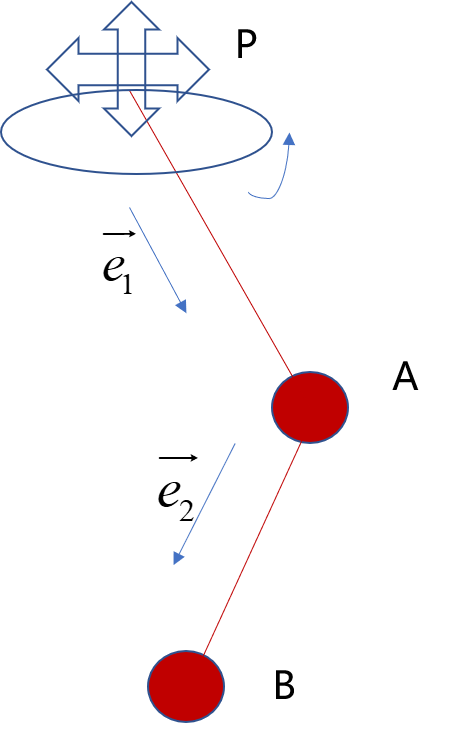
\includegraphics[scale=0.3]{T51.PNG}\
	
		\begin{figure}[h] %figure环境,h默认参数是可以浮动,不是固定在当前位置。如果要不浮动,你就可以使用大写float宏包的H参数,固定图片在当前位置,禁止浮动。
		\centering %使图片居中显示
		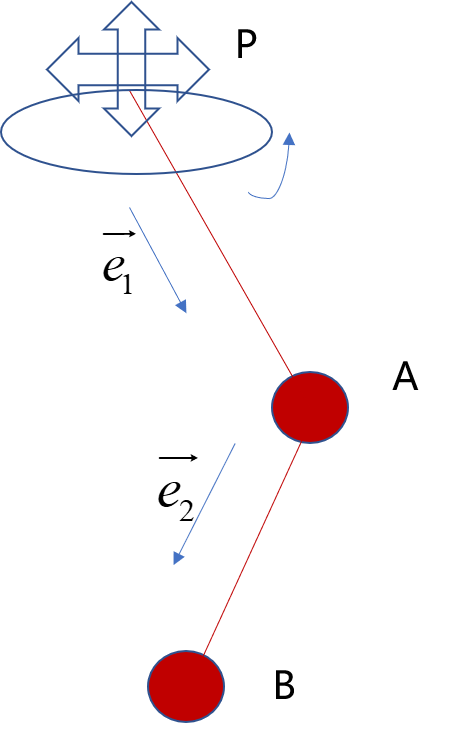
\includegraphics[height=8\baselineskip]{T51.PNG} %中括号中的参数是设置图片充满文档的大小,你也可以使用小数来缩小图片的尺寸。
		%\caption{狼伴归途} %caption是用来给图片加上图题的
		%\label{wolf} %这是添加标签,方便在文章中引用图片。
	\end{figure}%figure环境
	
	\noindent\textbf{因为中间球是穿在绳子上的,因此可以认为绳子上的拉力大小是一样的;此系统为哈密顿系统,我们采用保辛算法(Symplectic)迭代求解。}
	\clearpage
	\thispagestyle{empty}
	\subsubsection{蛙跳法原理介绍}
	\noindent\textbf{}
	
%	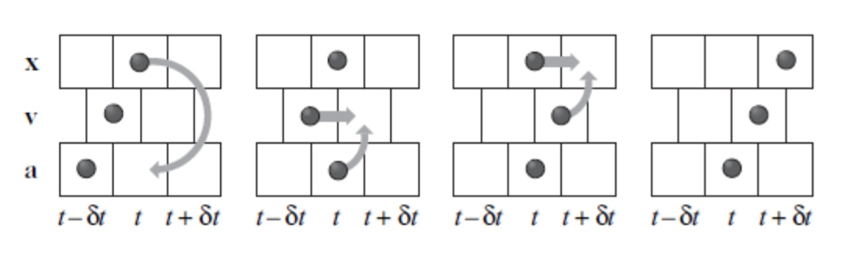
\includegraphics[scale=0.3]{T52.PNG}\
		\begin{figure}[h] %figure环境,h默认参数是可以浮动,不是固定在当前位置。如果要不浮动,你就可以使用大写float宏包的H参数,固定图片在当前位置,禁止浮动。
		\centering %使图片居中显示
		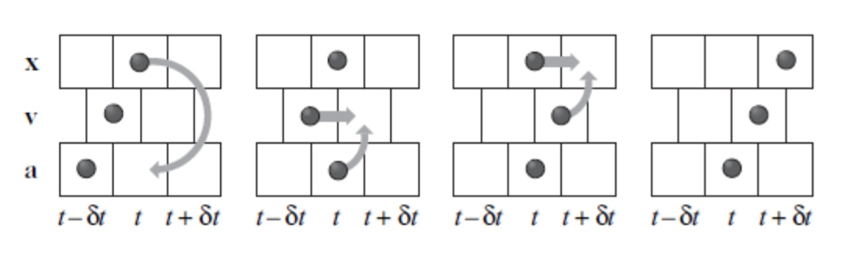
\includegraphics[height=8\baselineskip]{T52.PNG} %中括号中的参数是设置图片充满文档的大小,你也可以使用小数来缩小图片的尺寸。
		%\caption{狼伴归途} %caption是用来给图片加上图题的
		%\label{wolf} %这是添加标签,方便在文章中引用图片。
	\end{figure}%figure环境
	
	\noindent\textbf{\qquad 蛙跳法原理图示}\\\
	
积分的起点是t时刻的坐标x(t)和$t-\frac{1}{2}\delta t$时刻的速度$v(t-\frac{1}{2}\delta t)$
 
第一跳;青蛙(积分计算者的目光焦点)首先站在x(t)的位置上,根据坐标计算出粒子受力,自然推 出t时刻的加速度a(t),完成第一跳。 

第二跳:根据a(t)算出$t+\frac{1}{2}\delta t$时刻的速度。$v(t+\frac{1}{2}\delta t)= v(t-\frac{1}{2}\delta t)+a(t)\cdot \delta t$第二跳完成。 

第三跳:根据$t+\frac{1}{2}\delta t$时刻的速度计算t时刻的位置 $x(t+\delta t)=x(t)+v(t+\frac{1}{2}\delta t)\cdot \delta t$第三跳完成。
而t时刻的速度则用,$t-\frac{1}{2}\delta t$和$t+\frac{1}{2}\delta t$时刻的速度的平均即可。 
	\subsubsection{具体分析}
	\begin{minipage}[b]{0.65\linewidth}
		注意到,两球碰撞的情形;
		
		我们采取数值模拟中常用的策略,考虑球具较大的弹性系数;
		两球碰撞过程中具有微小的形变,借此计算其受力、加速度、位移变化。
		
		运动过程中,绳子会有一定程度上的伸长,根据伸长量和劲度系数计算两球受力;当绳长松弛时,绳子拉力为零;
		
	\end{minipage}
	\hfill
	\begin{minipage}[b]{0.35\linewidth}
		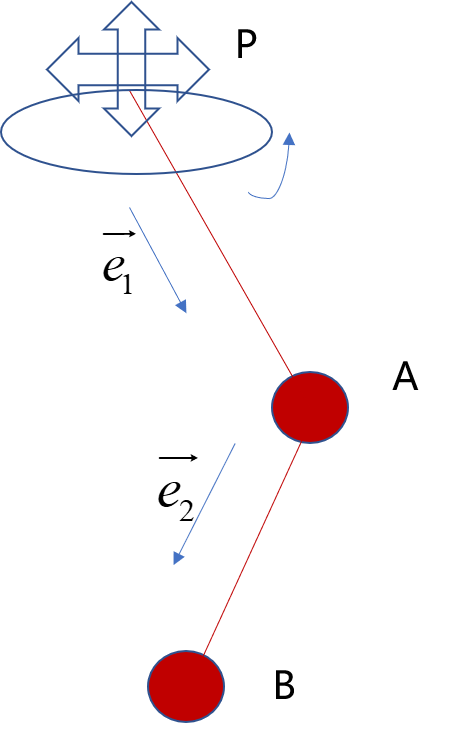
\includegraphics[height=8\baselineskip]{T51.PNG}
	\end{minipage}
	\clearpage
	\thispagestyle{empty}
	\subsection{建立方程}
	n: 代表第n个时间点;P:顶端球的位置;A:中间球位置;B:末端球位置;
	\noindent\textbf{}
	
	%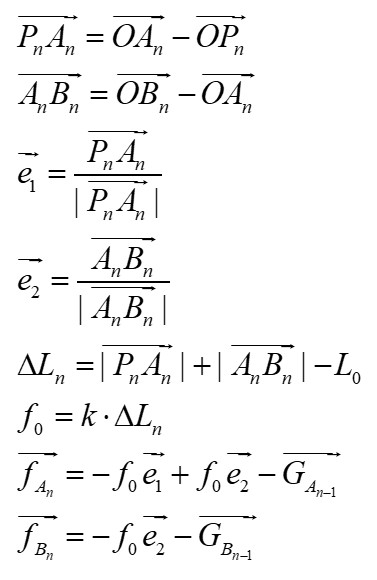
\includegraphics[scale=0.6]{T53.jpg}\
			\begin{figure}[h] %figure环境,h默认参数是可以浮动,不是固定在当前位置。如果要不浮动,你就可以使用大写float宏包的H参数,固定图片在当前位置,禁止浮动。
		\centering %使图片居中显示
		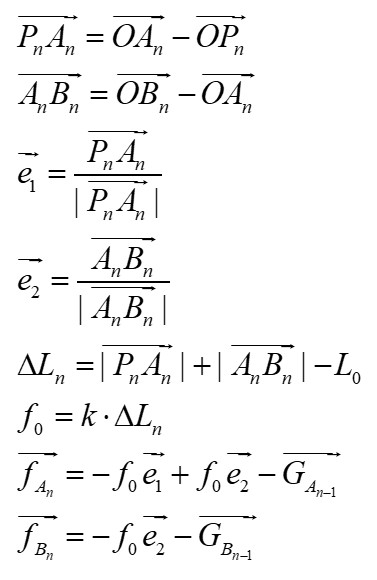
\includegraphics[scale=0.6]{T53.jpg} %中括号中的参数是设置图片充满文档的大小,你也可以使用小数来缩小图片的尺寸。
		%\caption{狼伴归途} %caption是用来给图片加上图题的
		%\label{wolf} %这是添加标签,方便在文章中引用图片。
	\end{figure}%figure环境
	\noindent\textbf{k劲度系数可由实验测得,绳子弹力大小}\\\
	\clearpage
	\thispagestyle{empty}
	
	采用“蛙跳法”迭代更新各个球的位置,速度,加速度。(注意到在此体系下)
	\begin{figure}[htb]
	\centering
	{
		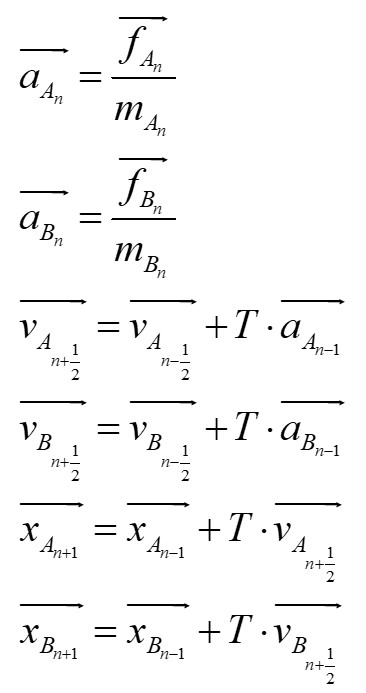
\includegraphics[width=4.5cm]{T54.jpg}}
	\hspace{0in}   
%	{
%		\includegraphics[width=6cm]{t51.png}}
%	\hspace{0in}

	\end{figure}
	\subsection{仿真误差分析}
		\begin{figure}[h] %figure环境,h默认参数是可以浮动,不是固定在当前位置。如果要不浮动,你就可以使用大写float宏包的H参数,固定图片在当前位置,禁止浮动。
	\centering %使图片居中显示
	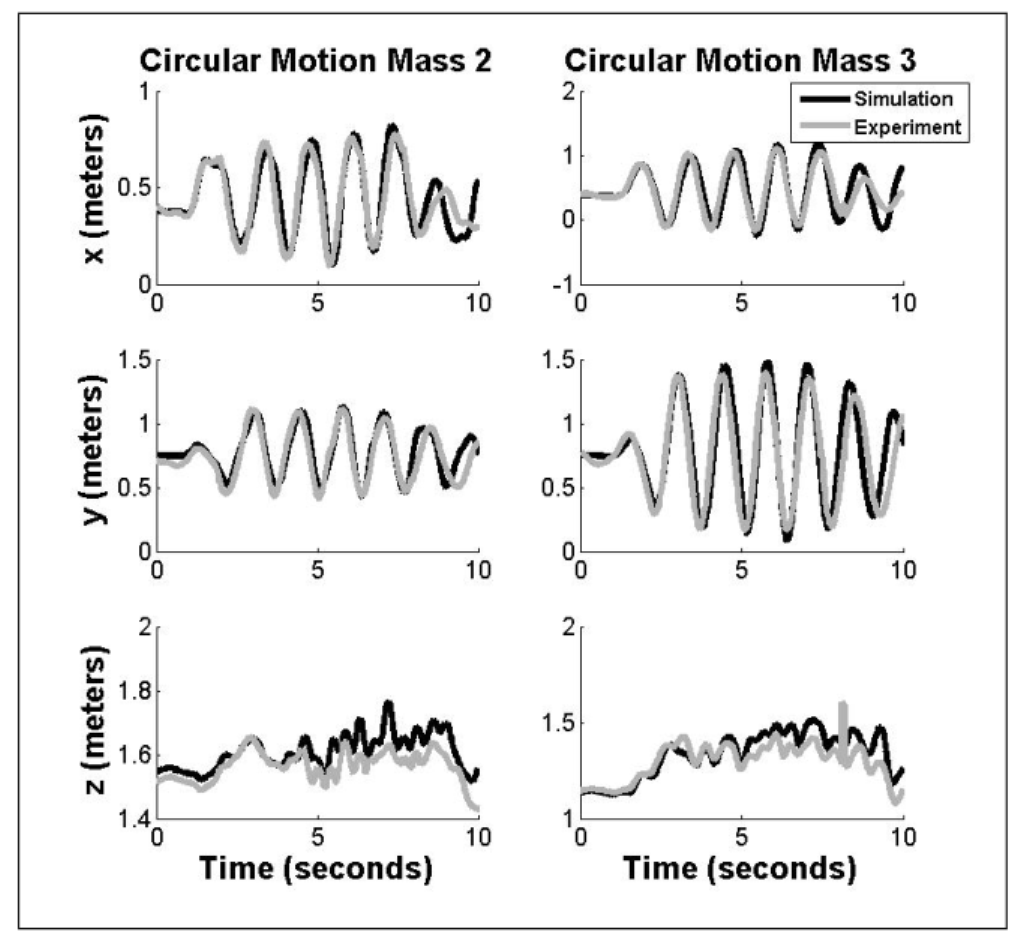
\includegraphics[height=16\baselineskip]{T098.jpg} %中括号中的参数是设置图片充满文档的大小,你也可以使用小数来缩小图片的尺寸。
	%\caption{中间球和底部球的位置随着时间演化仿真与实验对照} %caption是用来给图片加上图题的
	%\label{wolf} %这是添加标签,方便在文章中引用图片。
\end{figure}%figure环境
	如图所示为中间球和底部球的位置坐标随时间变化的仿真与实验对比图,我们先使用两台高速摄像机拍摄从一个特定位置无初速度释放后两球的运动轨迹,使用专业图像分析软件Tracker追踪并量化其位置坐标随时间变化,将小球的质量、绳子长度,劲度系数、空气阻尼系数和初始位置的坐标输入到仿真程序中,对比其坐标随时间的变化。通过上图我们发现,仿真与实验数据符合较好,在较长的演化时间内$MSE \leqslant 0.0001$
	
	
	\subsection{虚拟仿真优点}
	该仿真实验装置简便,可用手机端APP进行操作,在这个人手一机的时代,使用这样的手机文件可以让更多的人接触到这个在美国风靡的新型玩具。同时在正确的物理背景支撑下,所用的保辛算法又保证了实验数据测量的准确性、可靠性、对真实情况的高度拟合性,可以保证这个APP在运营期间容错率大大提高,保证用户的稳定体验,让用户在千百次的实验中得到稳定的数据保证。基于这些优势,预期可以成为教学成本低、操作难度小、实验结果直观可靠的教学工具,完全可以在教学期间用这样的工具
	%\clearpage
	%\thispagestyle{empty}
	\\
	\indent 作为实际玩具的替代品,不需要老师再去带一些额外的实验教学器材来辅助教学,可以仅用一台电脑来达到更高的教学效果,具有很大的推广价值。同时又因为其较高的性价比,应当可以为使用者带来可观的经济效益。而与此同时,我们认为作品已经的成熟,但从设计思路、使用的算法等方面还有一定改进的空间,我们在今后仍会不断完善这个作品。
%	\section{title}
	\section{附录}
	\subsection{windows平台操作}
		\begin{figure}[h] %figure环境,h默认参数是可以浮动,不是固定在当前位置。如果要不浮动,你就可以使用大写float宏包的H参数,固定图片在当前位置,禁止浮动。
		\centering %使图片居中显示
		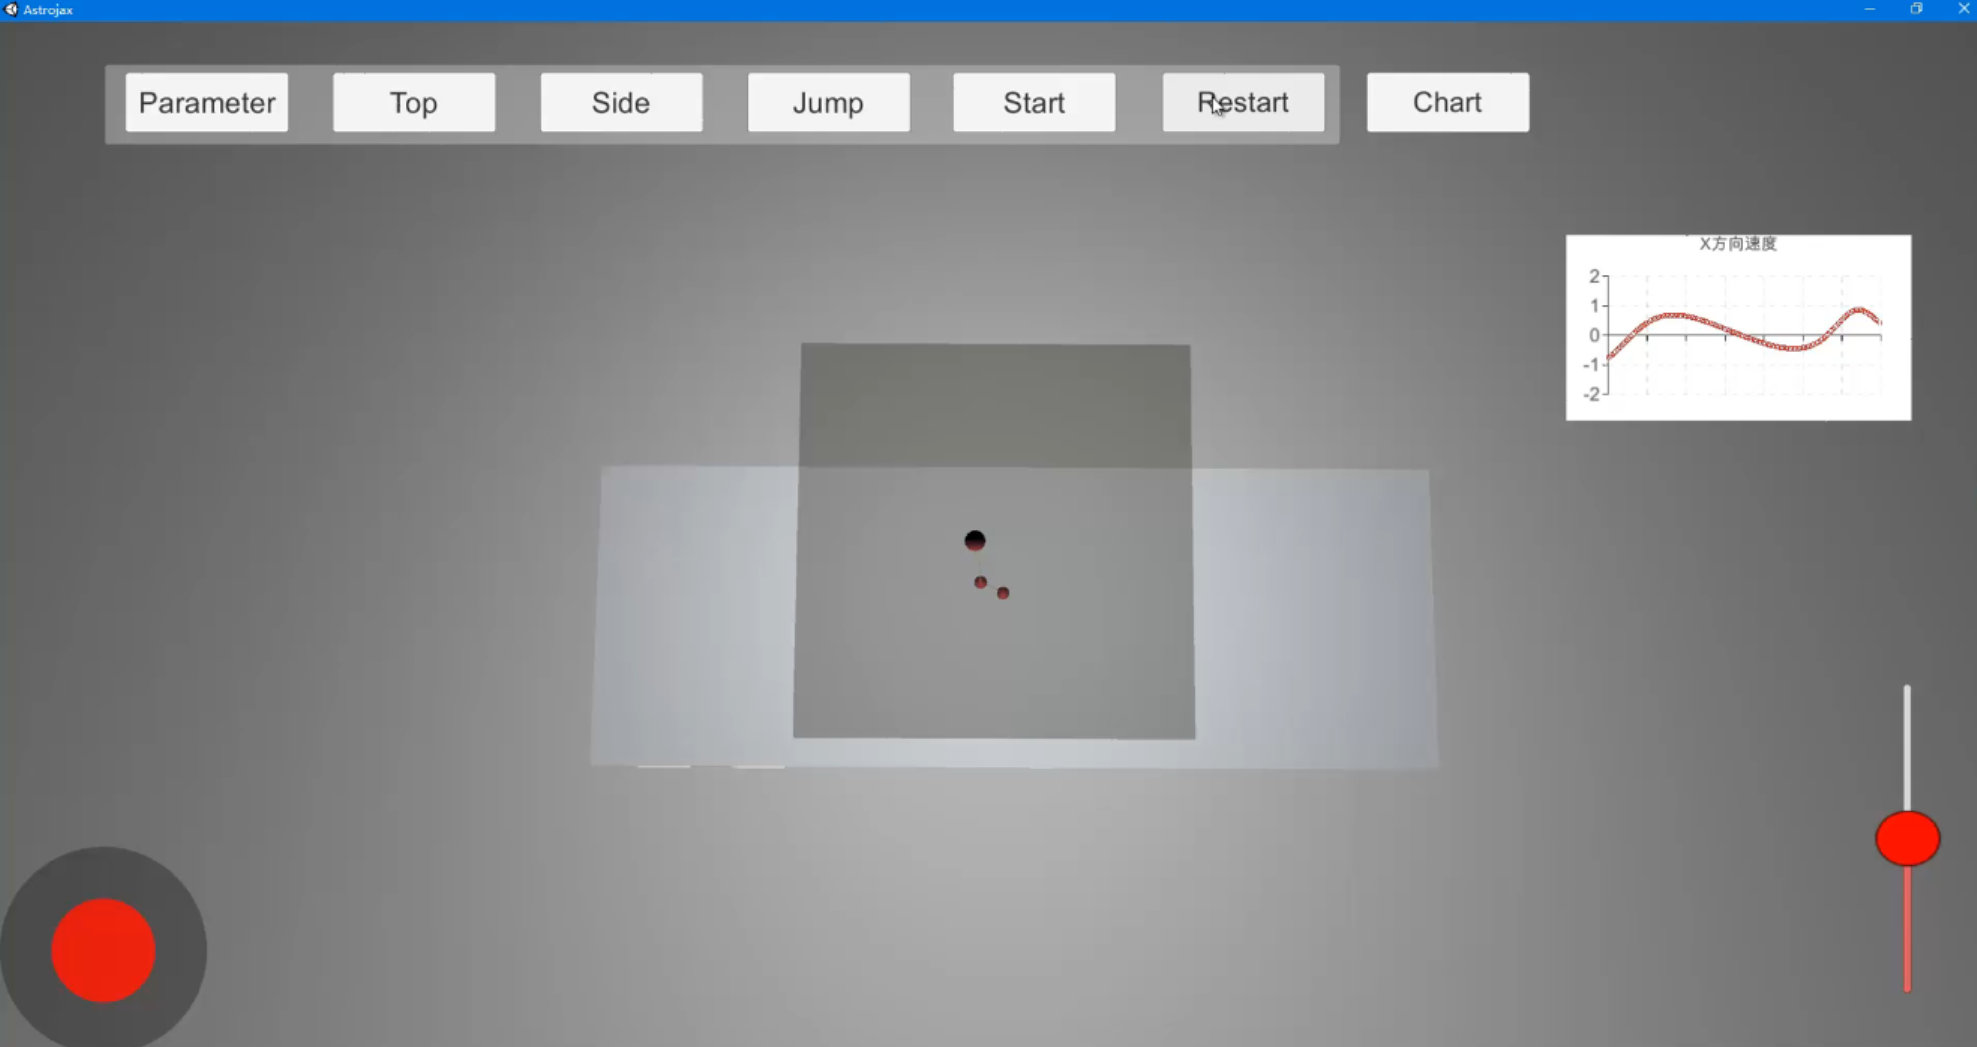
\includegraphics[scale=0.5]{T802.jpg} %中括号中的参数是设置图片充满文档的大小,你也可以使用小数来缩小图片的尺寸。
		%\caption{狼伴归途} %caption是用来给图片加上图题的
		%\label{wolf} %这是添加标签,方便在文章中引用图片。
	\end{figure}%figure环境
我们将仿真得出的运动轨迹与实验进行对比,发现在较长时间内,我们的仿真模型与实际符合较好。

借助仿真程序,可以把很多实验搬到大家的手机上。
虚拟仿真可以验证、展现出我们的理论分析。

同学可以在虚拟仿真中可以自己调节参数,探究出更多的稳定态。

如图为我们的仿真程序,
左下角的红色按钮类似于我们玩手机游戏时的操纵杆,可以控制最上端球的水平移动,而右下角的红色按钮,可以控制最上端球的竖直运动;
我们可以选择在不同的视角下观察系统的运动状态;
我们也可以导入数据,自己设定数据条件,即,自定义玩法;
右上角的曲线表示末端球在x方向上的速度随着时间的变化;。


	
	
	
	
\subsection{C \# 代码(部分)}
	
\begin{lstlisting}
using System.Collections;
using System.Collections.Generic;
using UnityEngine;
using UnityEngine.UI;
using System;
using System.IO;
using System.Text;
//using System.Diagnostics;

public class BallController : MonoBehaviour
{
// 图表组件
public SpeedChart chart;

private int nball;
private int ndyn;
private float dt;
private float k;
private float damping;
private float ks;
private float m;
private float g;
private float L0;
private float L1;
private float L2;
private float dL;
private float t;
private float driver_f;
private float driver_r;
private float driver_a;
private float driver_p;
private float L;
private float Fsr;
private float radius;
private float cradius;
private float diameter;
private float cdiameter;
private float amp;
private float force_radius;
private Vector3[] X;
private Vector3[] V;
private Vector3[] F;
private Vector3 Fs2;
private Vector3 Fs1;
private Vector3 Ft2;
private Vector3 Ft1;
private Vector3[,] F_pair;
private Vector3[] a;
private Vector3 e0;
private Vector3 e1;
private Vector3 e;
private Vector3 dX;
private Vector3 origin;
private Vector3 CX0;
private Vector3 CX1;
private float[,] Fr;
private float[,] D;
private List<GameObject> balls;
private List<MoveController> ballscripts;
private List<GameObject> strings;
private List<MoveString> stringscripts;
public GameObject Ballpref;
public GameObject Stringpref;

// Start is called before the first frame update
void Start()
{
Initiate_params();

for (int i = 0; i < nball; i++)

MoveController ballscript = newBall.GetComponent<MoveController>();
balls.Add(newBall.gameObject);
ballscripts.Add(ballscript);
}

for (int i = 0; i < 2; i++)
{
GameObject newString = Instantiate(Stringpref);
newString.transform.localScale = new Vector3(10.0f, 10.0f, 10.0f);
MoveString stringscript = newString.GetComponent<MoveString>();
strings.Add(newString.gameObject);
stringscripts.Add(stringscript);
}

Initiate_xv();

UpdatePos();
}

public void Run()
{
Get_xv();
Distance();
//L0 = L;
Get_bond();


InvokeRepeating("UpdatePos", 0f, 0.01f);
}

void UpdatePos()
{

Get_xv();
Update_xv(nball, X, V, dt, ndyn, 1);
//Debug.Log("L0 = " + L0);
//Debug.Log("L  = " + L );
Set_xv();
Update_position();

// 更新图表
chart.AddData("",V[2].x);

if (Input.GetKey(KeyCode.Escape))
{
Screen.fullScreen = false;  //退出全屏         
}
//按A全屏
if (Input.GetKey(KeyCode.A))
{
Screen.SetResolution(1920, 1080, true);
Screen.fullScreen = true;  //设置成全屏
}

}
{
origin = new Vector3(0.0f, 0.0f, 0.0f);
if (key == "dp")
{
damping = float.Parse(value);
}
else if (key == "l0")
{
L0 = float.Parse(value);
}
else if (key == "g")
{
g = float.Parse(value);
}
else if (key == "X0x")
{
ballscripts[0].x.x = float.Parse(value) + origin.x;
}
else if (key == "X0y")
{
ballscripts[0].x.y = float.Parse(value) + origin.y;
}
else if (key == "X0z")
{
ballscripts[0].x.z = float.Parse(value) + origin.z;
}
else if (key == "X1x")
{
ballscripts[1].x.x = float.Parse(value) + origin.x;
}
else if (key == "X1y")
{
ballscripts[1].x.y = float.Parse(value) + origin.y;
}
else if (key == "X1z")
{
ballscripts[1].x.z = float.Parse(value) + origin.z;
}
else if (key == "X2x")
{
ballscripts[2].x.x = float.Parse(value) + origin.x;
}
else if (key == "X2y")
{
ballscripts[2].x.y = float.Parse(value) + origin.y;
}
else if (key == "X2z")
{
ballscripts[2].x.z = float.Parse(value) + origin.z;
}
else if (key == "V0x")
{
ballscripts[0].v.x = float.Parse(value);
}
else if (key == "V0y")
{
ballscripts[0].v.y = float.Parse(value);
}
else if (key == "V0z")
{
ballscripts[0].v.z = float.Parse(value);
}
else if (key == "V1x")
{
ballscripts[1].v.x = float.Parse(value);
}
else if (key == "V1y")
{
ballscripts[1].v.y = float.Parse(value);
}
else if (key == "V1z")
{
ballscripts[1].v.z = float.Parse(value);
}
else if (key == "V2x")
{
ballscripts[2].v.x = float.Parse(value);
}
else if (key == "V2y")
{
ballscripts[2].v.y = float.Parse(value);
}
else if (key == "V2z")
{
ballscripts[2].v.z = float.Parse(value);
}
Get_xv();

{
ballscripts[0].x.y = value * 0.1f;
}
public void ChangeXZ(float xratio, float yratio)
{
float x0 = -0.2f;
float z0 = -0.2f;
float wid = 0.4f;
float hei = 0.4f;
ballscripts[0].x.x = x0 + wid * xratio;
ballscripts[0].x.z = z0 + hei * yratio;

}


public void Jump(Vector3 pos)
{
//X[0].y += 5;
ballscripts[0].x.y = pos.y * 0.1f;

}

//---------------------------------------------------------
void Initiate_params()
{
//---------------------------------------------------------
// Initiation
//
nball = 3;
ndyn = 20;
dt = 0.0001f;
radius = 0.01f;
cradius = radius / 5.0f;
diameter = radius * 2.0f;
cdiameter = cradius * 2.0f;
damping = 0.005f;
//driver_f = 0.1f;
driver_f = 1.0f;
//driver_r = 2.0f;
driver_p = 0.0f;
//amp = 0.1f;
t = 0.0f;
//damping = 0.000f;
//driver_f = 0.0f;
//driver_r = 0.0f;
k = 28000.0f;
ks = 28000.0f;
m = 31.88f;
m = m / 1000.0f;
g = 9.8f;
// g = g * 0.01f;
force_radius = 2.0f * radius;
L0 = 0.61f;
//
balls = new List<GameObject>();
ballscripts = new List<MoveController>();
strings = new List<GameObject>();
stringscripts = new List<MoveString>();

e = new Vector3();
origin = new Vector3();
dX = new Vector3();
e0 = new Vector3();
e1 = new Vector3();
CX0 = new Vector3();
CX1 = new Vector3();
Fs2 = new Vector3();
Fs1 = new Vector3();
Ft2 = new Vector3();
Ft1 = new Vector3();
X = new Vector3[nball];
V = new Vector3[nball];
a = new Vector3[nball];
F = new Vector3[nball];
F_pair = new Vector3[nball, nball];
D = new float[nball, nball];
Fr = new float[nball, nball];
}

}
void Get_xv()
{
for (int i = 0; i < nball; i++)
{
X[i] = ballscripts[i].x;
V[i] = ballscripts[i].v;
}
}
void Set_xv()
{
for (int i = 0; i < nball; i++)
{
ballscripts[i].x = X[i];
ballscripts[i].v = V[i];
}
}
void Update_position()
{
for (int i = 0; i < nball; i++)
{
balls[i].transform.position = ballscripts[i].x;
}
}
void Distance()
{
for (int i = 0; i < nball; i++)
{
for (int j = i+1; j < nball; j++)
{
if (i == j)
{
D[i, j] = 0.0f;
}
else
{
D[i, j] = (X[i] - X[j]).magnitude;
D[j, i] = D[i, j];
}
}
}
L1 = D[0, 1];
L2 = D[1, 2];
L = L1 + L2;
}

{
for (int i = 0; i < nball - 1; i++)
{
for (int j = i + 1; j < nball; j++)
{
if (D[i, j] < force_radius)
{
float dr = force_radius - D[i, j];
Fr[i, j] = k * dr;
}
else
{
Fr[i, j] = 0.0f;
}
e = (X[i] - X[j]) / D[i, j];
// The force act on i
F_pair[i, j] = e * Fr[i, j];
// The force act on j
F_pair[j, i] = -F_pair[i, j];
}
}

for (int i = 0; i < N; i++)
{
V[i].x = V[i].x + a[i].x * dt / 2.0f; 
V[i].y = V[i].y + a[i].y * dt / 2.0f;
V[i].z = V[i].z + a[i].z * dt / 2.0f;
}
//----------------------------------------------------------
for (int i = 0; i < N; i++)
{
t = t + dt;
if (i == -1)
{
if (driver_f > 0.0f) {
//driver_a = driver_f * dt;
driver_a = driver_f * t;
dX = new Vector3(0.0f, 0.0f, 0.0f);
//----------------------------------------------------------

// move along y axis
//
// dX.y = amp * (float)Math.Cos(driver_a + driver_p);
dX.y = amp * (float)Math.Cos(driver_a);
UnityEngine.Debug.Log(driver_f);
UnityEngine.Debug.Log(dt);
//----------------------------------------------------------
// X[i] = origin + dX;
}
}
else
{
X[i].x = X[i].x + V[i].x * dt;
X[i].y = X[i].y + V[i].y * dt;
X[i].z = X[i].z + V[i].z * dt;
}
}
//-------------------------------------------------------------
Cal_force();
//-------------------------------------------------------------
for (int i = 0; i < N; i++)
{
V[i].x = V[i].x + a[i].x * dt / 2.0f;
V[i].y = V[i].y + a[i].y * dt / 2.0f;
V[i].z = V[i].z + a[i].z * dt / 2.0f;
//------------------------------------------------------------
}
Get_bond();
}
}


// Update is called once per frame
void Update()
{


}


}


	\end{lstlisting}
		\subsection{Python代码(部分)}

	\begin{lstlisting}[language=Python]
import numpy as np 
import matplotlib as mpl
import matplotlib.pyplot as plt
from mpl_toolkits.mplot3d import Axes3D
	
#定义基本物理量,M表示质量,T为时间间隔;
#x为位置,v为速度,g为重力系数,k为绳子张力系数
Ma = 0.1
Mb = 0.1
g = 9.8
T = 0.0001
k = 1000
x0 = np.asarray([0.0 , 0.0, 0.0])
xa = np.asarray([0.5 , 0, 0])
xb = np.asarray([1.0 , 0, 0]) 
va = np.asarray([0.0 , 0.0, 0.0])
vb = np.asarray([0.0 , 0.0, 0.0])
l0a = (np.sum((xa - x0) ** 2)) ** 0.5
lab = (np.sum((xa - xb) ** 2)) ** 0.5
l0 = l0a + lab
print(x0,xa,xb,l0a,lab)
def fun(x0,xa,xb,va,vb):
#确定受力大小
disab = (np.sum((xa - xb) ** 2)) ** 0.5
dis0a = (np.sum((xa - x0) ** 2)) ** 0.5
dis0 = disab + dis0aC
# if disab - lab > 0:
#     fab = k * (disab - lab) #  
# else :
#     fab = 0
	
# if dis0a - l0a > 0:
#     f0a = k * (dis0a - l0a)
# else:
#     f0a = 0
	
if dis0 - l0 > 0:
f0 = k * (dis0 - l0)
else:
f0 = 0
#确定受力方向并归一化
vec0a = xa - x0
vecba = xa - xb
vec0a = vec0a / (np.sum(vec0a ** 2)) ** 0.5
vecba = vecba / (np.sum(vecba ** 2)) ** 0.5
fa = -vec0a * f0 - vecba * f0 +  np.asarray([0, 0, -Ma * g])
fb = vecba * f0 + np.asarray([0, 0, -Mb * g])
#确定加速度
a_a = fa / Ma
a_b = fb / Mb
#执行移动模块并
va = va + a_a * T
vb = vb + a_b * T
xa = xa + va * T
xb = xb + vb * T
	
return xa,xb,va,vb
	
num = 0
x1 = []
y1 = []
z1 = []
x2 = []
y2 = []
z2 = []
N = 100
	
Tx0 = []
theta = 0
for i in range(N):
x = 0.0*np.asarray([np.sin(theta),np.cos(theta),0])
Tx0.append(x)
theta = theta + 0.01
while num < N:
xa,xb,va,vb = fun(Tx0[num],xa,xb,va,vb)
x1.append(xa[0])	
y1.append(xa[1])
z1.append(xa[2])
x2.append(xb[0])
y2.append(xb[1])
z2.append(xb[2])
num = num + 1
vec0a = xa - x0
vecba = xa - xb
t = (np.sum(vec0a ** 2)) ** 0.5 + (np.sum(vecba ** 2)) ** 0.5
print(t)
# mpl.rcParams['legend.fontsize'] = 10

	
	
	
	
	
	\end{lstlisting}
\end{document}
	